\section{About the EROS training set}

We use a training data set provided by \citet{kim2014} which contains labels (main and sub--classes) and lightcurves for $32655$ sources in the Large Magellanic Cloud (LMC). The lightcurves were recorded by the Expérience pour la Recherche d’Objets Sombres (EROS) project, a wide--field survey. A thorough description of the compilation process is available in \citet{kim2014}, however, here is a list of the main steps:

\begin{enumerate}
\item Compile known periodoic variables in the LMC from the OGLE and MACHO surveys
\item Add $982$ blue variables (BVs) from the MACHO database
\item Add 565 quasi--stellar objects (QSOs)
\item 
\end{enumerate}

% Number of sources in the data set
% Not a standard astronomical B and R bands

\section{Feature Extraction}

We extract a variety of features characterizing the variability of the source. A lot of them are standard statistical features, but some are more sophisticated, trying to incorporate a model of the underlying physics. In the following, $N$ will be the number of data points in the light curve, $(t_i, m_i)$ the $i^{\text{th}}$ data point in the light curve. Some of the features are extracted from the recorded lightcurve, as well as from the phase--folded lightcurve ($P_{\text{LS}}$). We label the latter with a superscript $\phi$, \eg $\mu^\phi, \sigma^\phi$ and so forth.

\begin{enumerate}
%\setlength{\itemsep}{5pt}
%\setlength{\parskip}{0pt}
%\setlength{\parsep}{0pt}
%\setlength{\abovedisplayskip}{.5em}
%\setlength{\belowdisplayskip}{.5em}

\litem{$\mu, \mu^\phi$ (Mean of magnitude)} The arithmetic mean of the magnitude, given by
\begin{equation}\mu = \frac{1}{N} \sum\limits_{i=1}^{N} m_i.\end{equation}

\litem{$\sigma, \sigma^\phi$ (Standard deviation of magnitude)} The standard deviation of the magnitude, given by
\begin{equation}\sigma = \sqrt{\frac{1}{N-1} \sum_{i=1}^N (m_i - \mu)^2}.\end{equation}

\litem{$Q_{50}, Q_{50}^\phi$ (Median of magnitude)} The median of the magnitude, given by
\begin{equation}Q_{50} = \cdots.\end{equation}

\litem{$\bar \mu, \bar \mu^\phi$ (Weighted mean of magnitude)} The weighted arithmetic mean of the magnitude, given by
\begin{equation}\bar \mu = \big(\sum\limits_{i=1}^{N} w_i m_i\big) \; / \; \big(\sum\limits_{i=1}^{N} w_i\big),\end{equation}
with weights $w_i$ inversely proportional to the measurement uncertainty, \ie $w_i = \sigma_i^{-1}$ with $\sigma_i > 0 \; \forall i$.

% Mention measurement uncertainty must be non-zero

\litem{$\bar \sigma, \bar \sigma^\phi$ (Weighted standard deviation of magnitude)} The weighted standard deviation of the magnitude, given by
\begin{equation}\bar \sigma = \sqrt{\frac{1}{(N-1) \sum\limits_{i=1}^{N} w_i} \sum_{i=1}^N w_i \, ( m_i - \bar \mu)^2}.\end{equation}
% @TODO: Specify weights
% @TODO: Add formula for weighted standard deviation

\litem{$\gamma_1, \gamma_1^\phi$ (Skewness)} The skewness of the magnitude, given by
\begin{equation}\gamma_1 = \frac{N}{(N-1)(N-2)} \sum\limits_{i=1}^N \big( \frac{m_i - \mu}{\sigma} \big)^3.\end{equation}

\litem{$\gamma_2, \gamma_2^\phi$ (Kurtosis)} The kurtosis of the magnitude, given by
\begin{equation}\gamma_2 = \frac{N(N+1)}{(N-1)(N-2)(N-3)} \sum\limits_{i=1}^N \big( \frac{m_i - \mu}{\sigma} \big)^4 - 3 \, \frac{(N-1)^2}{(N-2)(N-3)}.\end{equation}

\litem{$Q_{25}, Q_{25}^\phi$ (25\% quartile)} The 25\% quartile of the magnitude, given by
\begin{equation}Q_{25} = \cdots.\end{equation}

\litem{$Q_{75}, Q_{75}^\phi$ (75\% quartile)} The 75\% quartile of the magnitude, given by
\begin{equation}Q_{75} = \cdots.\end{equation}

\litem{$\text{IQR}, \text{IQR}^\phi$ (Interquartile range)} The interquartile range of the magnitude, given by
\begin{equation}\text{IQR} = Q_{75} -Q_{25}.\end{equation}

\litem{$P_{\text{LS}}$ (Lomb--Scargle period)} The period of the signal according to the Lomb--Scargle algorithm, given by
\begin{equation}P_{\text{LS}} = \frac{1}{2 \sigma_y^2} \Bigg\{ \frac{\big[\sum\limits_{i=1}^k (y_i - \mu_y) \cos(\omega(t_i - \tau))\big]^2}{\sum\limits_{i=1}^k \cos^2(\omega(t_i - \tau))} + \frac{\big[\sum\limits_{i=1}^k (y_i - \mu_y) \sin(\omega(t_i - \tau))\big]^2}{\sum\limits_{i=1}^k \sin^2(\omega(t_i - \tau))}\Bigg\}\end{equation}

\litem{$\text{FAP}_{\text{LS}}$ (False--Alarm probability for Lomb--Scargle)} The false--alarm probability (FAP) for the Lomb--Scargle algorithm, given by
\begin{equation}\text{FAP}_{\text{LS}}(x) = 1 - (1 - \euler^{-x})^M.\end{equation}

\litem{$\text{SNR}, \text{SNR}^\phi$ (Signal--to--noise ratio)} The signal--to--noise ratio, given by
\begin{equation}\text{SNR} = \frac{\mu}{\sigma}.\end{equation}

\litem{$S, S^\phi$ (Shannon entropy)} The Shannon entropy of the signal, given by
\begin{equation}S = -\sum\limits_{i=1}^N m_i \ln(m_i).\end{equation}

\litem{$\eta, \eta^\phi$ (Eta--feature)} The $\eta$ feature as proposed by \citep{}, given by
\begin{equation}\eta = \frac{1}{\sigma^2 (N-1)} \sum\limits_{i=1}^{N-1} (m_{i+1} - m_{i})^2.\end{equation}

\litem{$\cdots$ (Half--magnitude--amplitude ratio)} The ratio of higher \resp lower amplitudes than average, given by
\begin{equation}\cdots = \sqrt{ \Big(\sum\limits_{l=1}^N \big( \alpha^{>}_l - \mu \big)^2\Big) \, / \, \Big(\sum\limits_{m=1}^N \big( \alpha^{<}_m - \mu \big)^2\Big)},\end{equation}
where $\alpha^{>}, \alpha^{<}$ are magnitudes higher resp. lower than $\mu$.

\litem{$\text{MAD}^{(1)}$ (Mean absolute deviation)} The mean absolute deviation of the magnitude, given by
\begin{equation}\text{MAD}^{(1)} = \cdots.\end{equation}

\litem{$\text{MAD}^{(2)}$ (Median absolute deviation)} The median absolute deviation of the magnitude, given by
\begin{equation}\text{MAD}^{(2)} = \cdots.\end{equation}

\litem{$\text{SF}$ (Structure function features)} We extract $A, \sigma_A, \gamma, \sigma_\gamma$ from the structure function power--law fit, given by
\begin{equation}\text{SF}(\Delta t) = \cdots.\end{equation}

\litem{$\mathcal{F}$ (Fourier features)} We fit standard fourier series with five terms to the phase--folded lightcurve.
\begin{equation}\mathcal{F}(t) = \frac{A_0}{2} + \sum_{k=1}^{\infty} ( A_k \cos(2 \pi k t) + B_k \sin(2 \pi k t) ).\end{equation}
From this we the extract amplitude and phase features $A_0$, $A_i = \sqrt{a_i^2 + b_i^2}$ and $\varphi_i = \arctan(\frac{b_i}{a_i})$ features for $i = 1, \ldots, 5$.

% CE – three candidate periods + scores
% sf-A-error, sf-gamma-error
% Slope percentile features
% fourier-A-i, fourier-phi-i
% fourier-residuals

% Shapiro-W und Shapiro-p
% Proper citing of all equations

\end{enumerate}

This leads to a total of $\cdots$ features in $\cdots$ bands.

% State that feature are highly correlated
% Show histogram of some features.
% Show some scatterplots
% More about period finding

\section{Performance of the Support Vector Machine}

The first classifier we try is the Support Vector Machine (SVM) with the RBF kernel $\kernel_{\text{RBF}}$. We optimize the models hyperparameters $C$ and $\gamma$ for the average, weighted $F_1$-score by performing a $5$-fold cross--validation on subsequently finer grids. The results are visualized in figure \ref{fig:gridsearch-svm-superclasses}.

\begin{figure}[H]
\subfigure{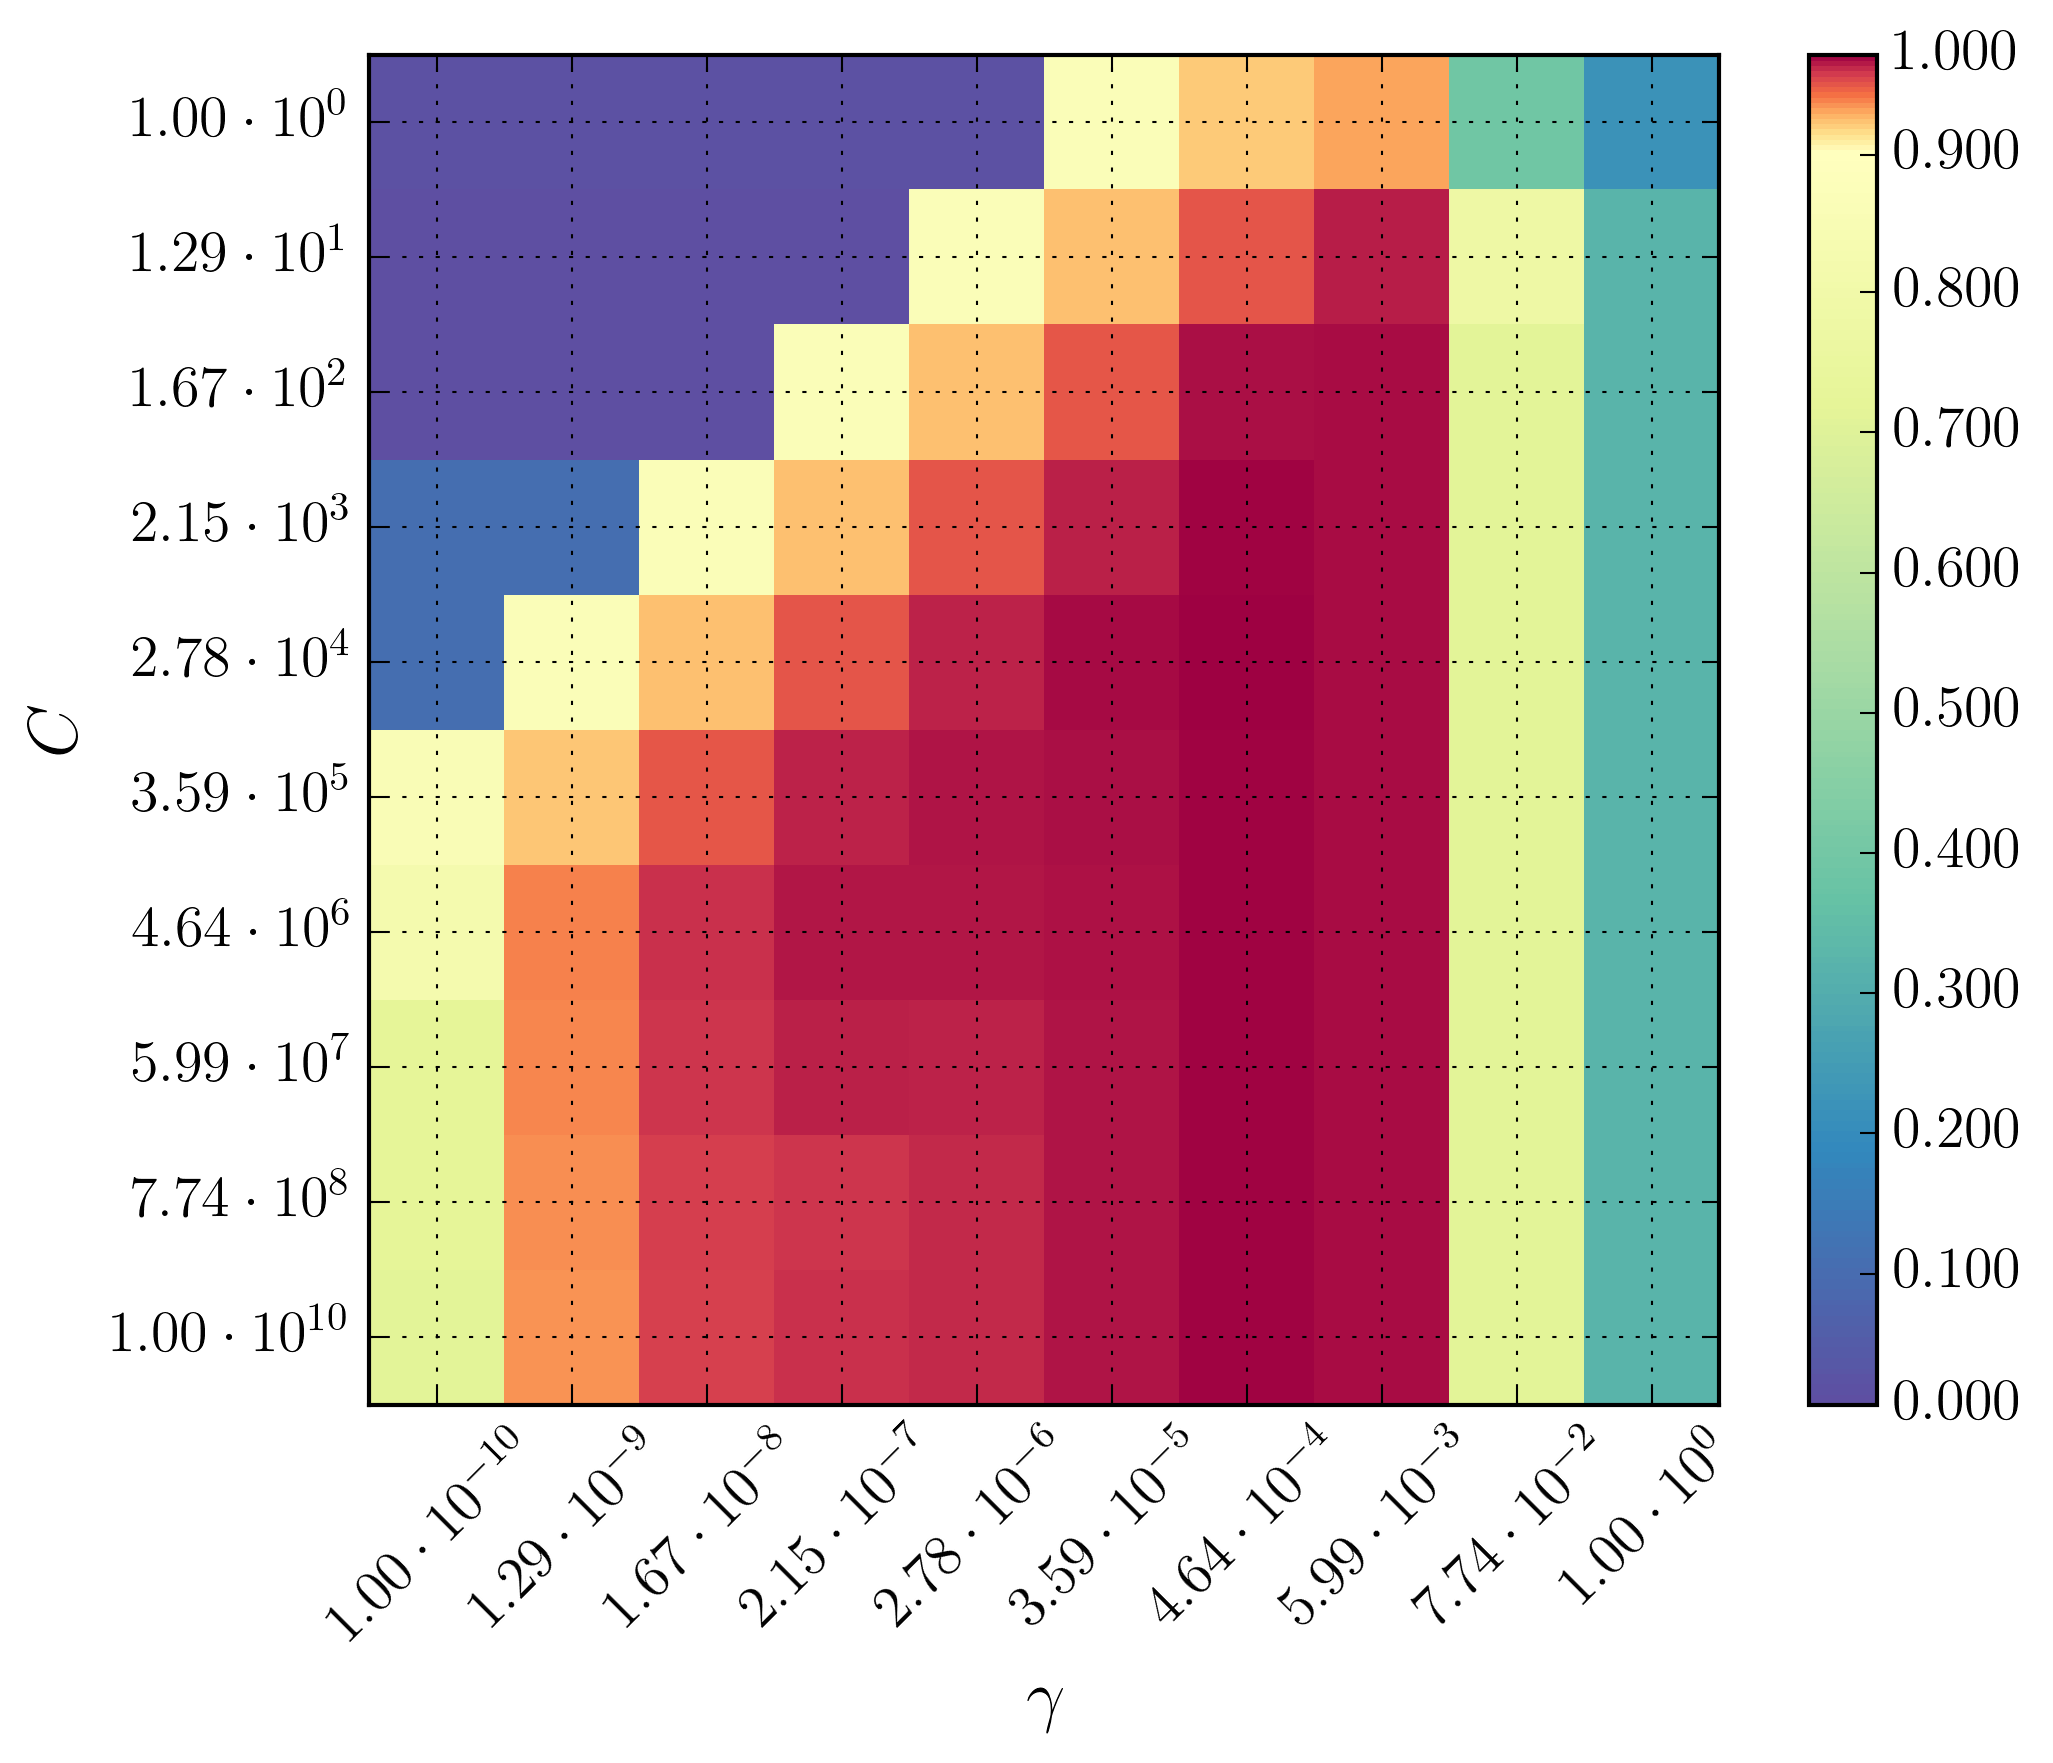
\includegraphics[width=0.49\textwidth,height=0.4\textwidth]{figures/gridsearch/svm/superclasses/svm-superclasses-01.png}}
\hfill
\subfigure{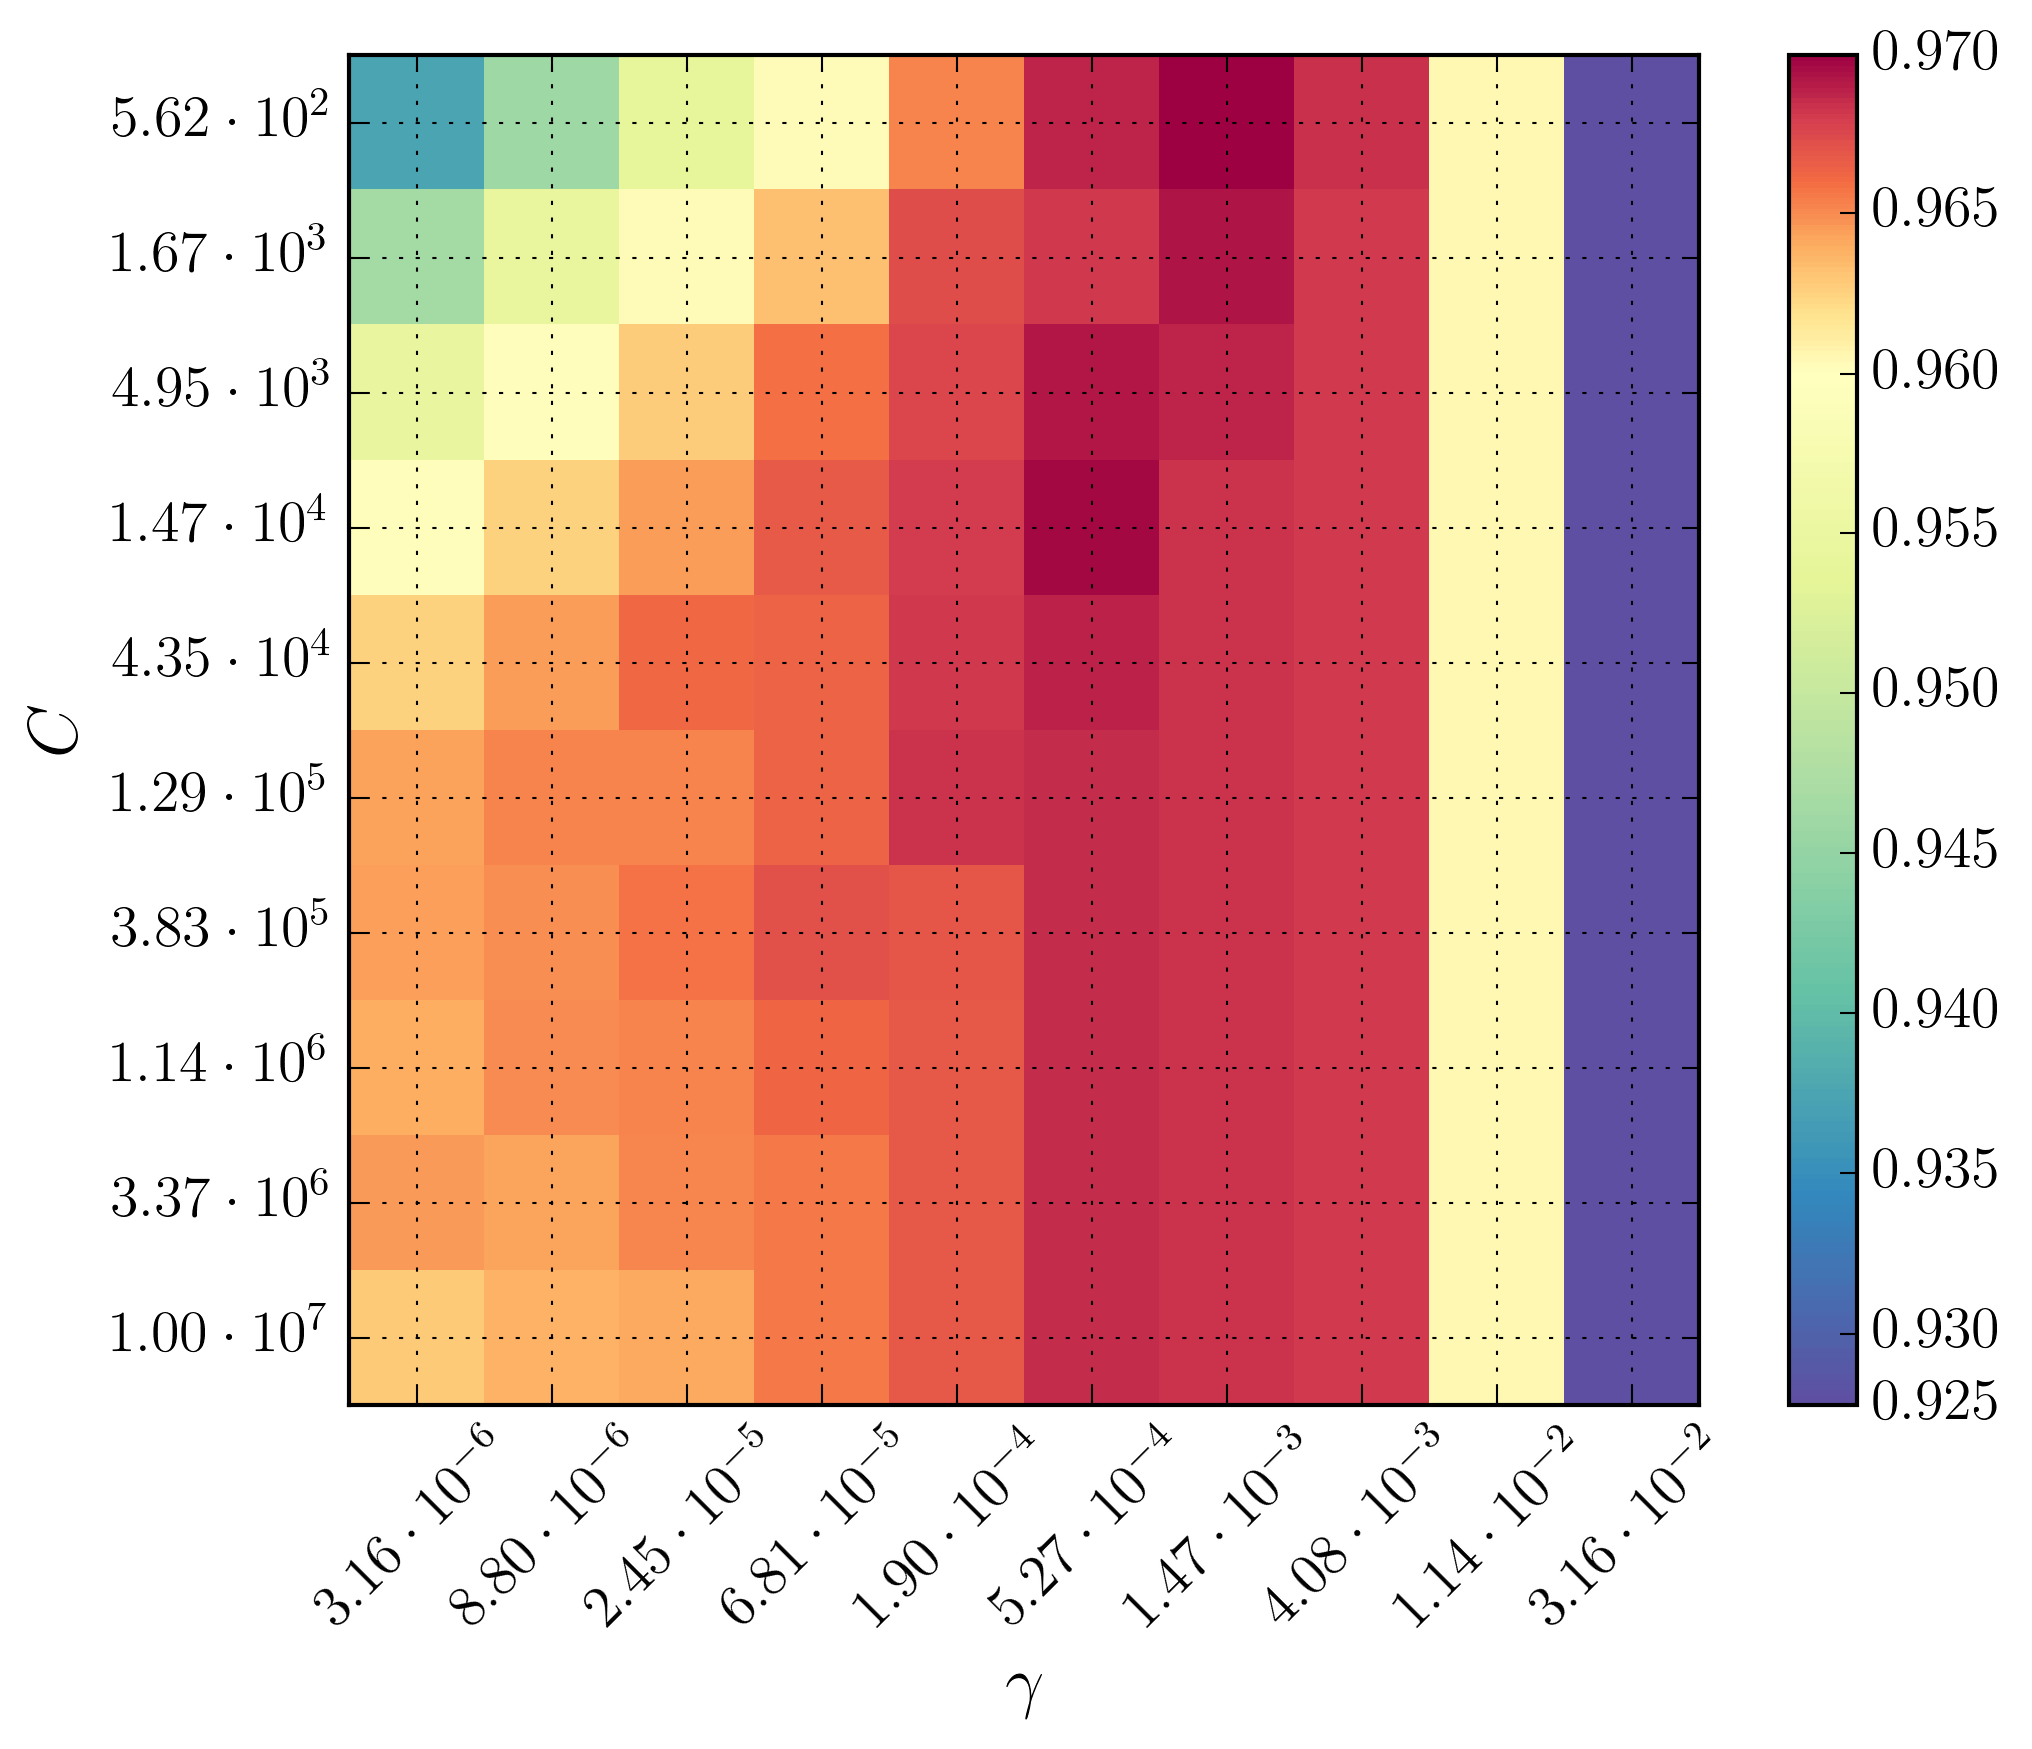
\includegraphics[width=0.51\textwidth,height=0.4\textwidth]{figures/gridsearch/svm/superclasses/svm-superclasses-02.png}}
\hfill
\subfigure{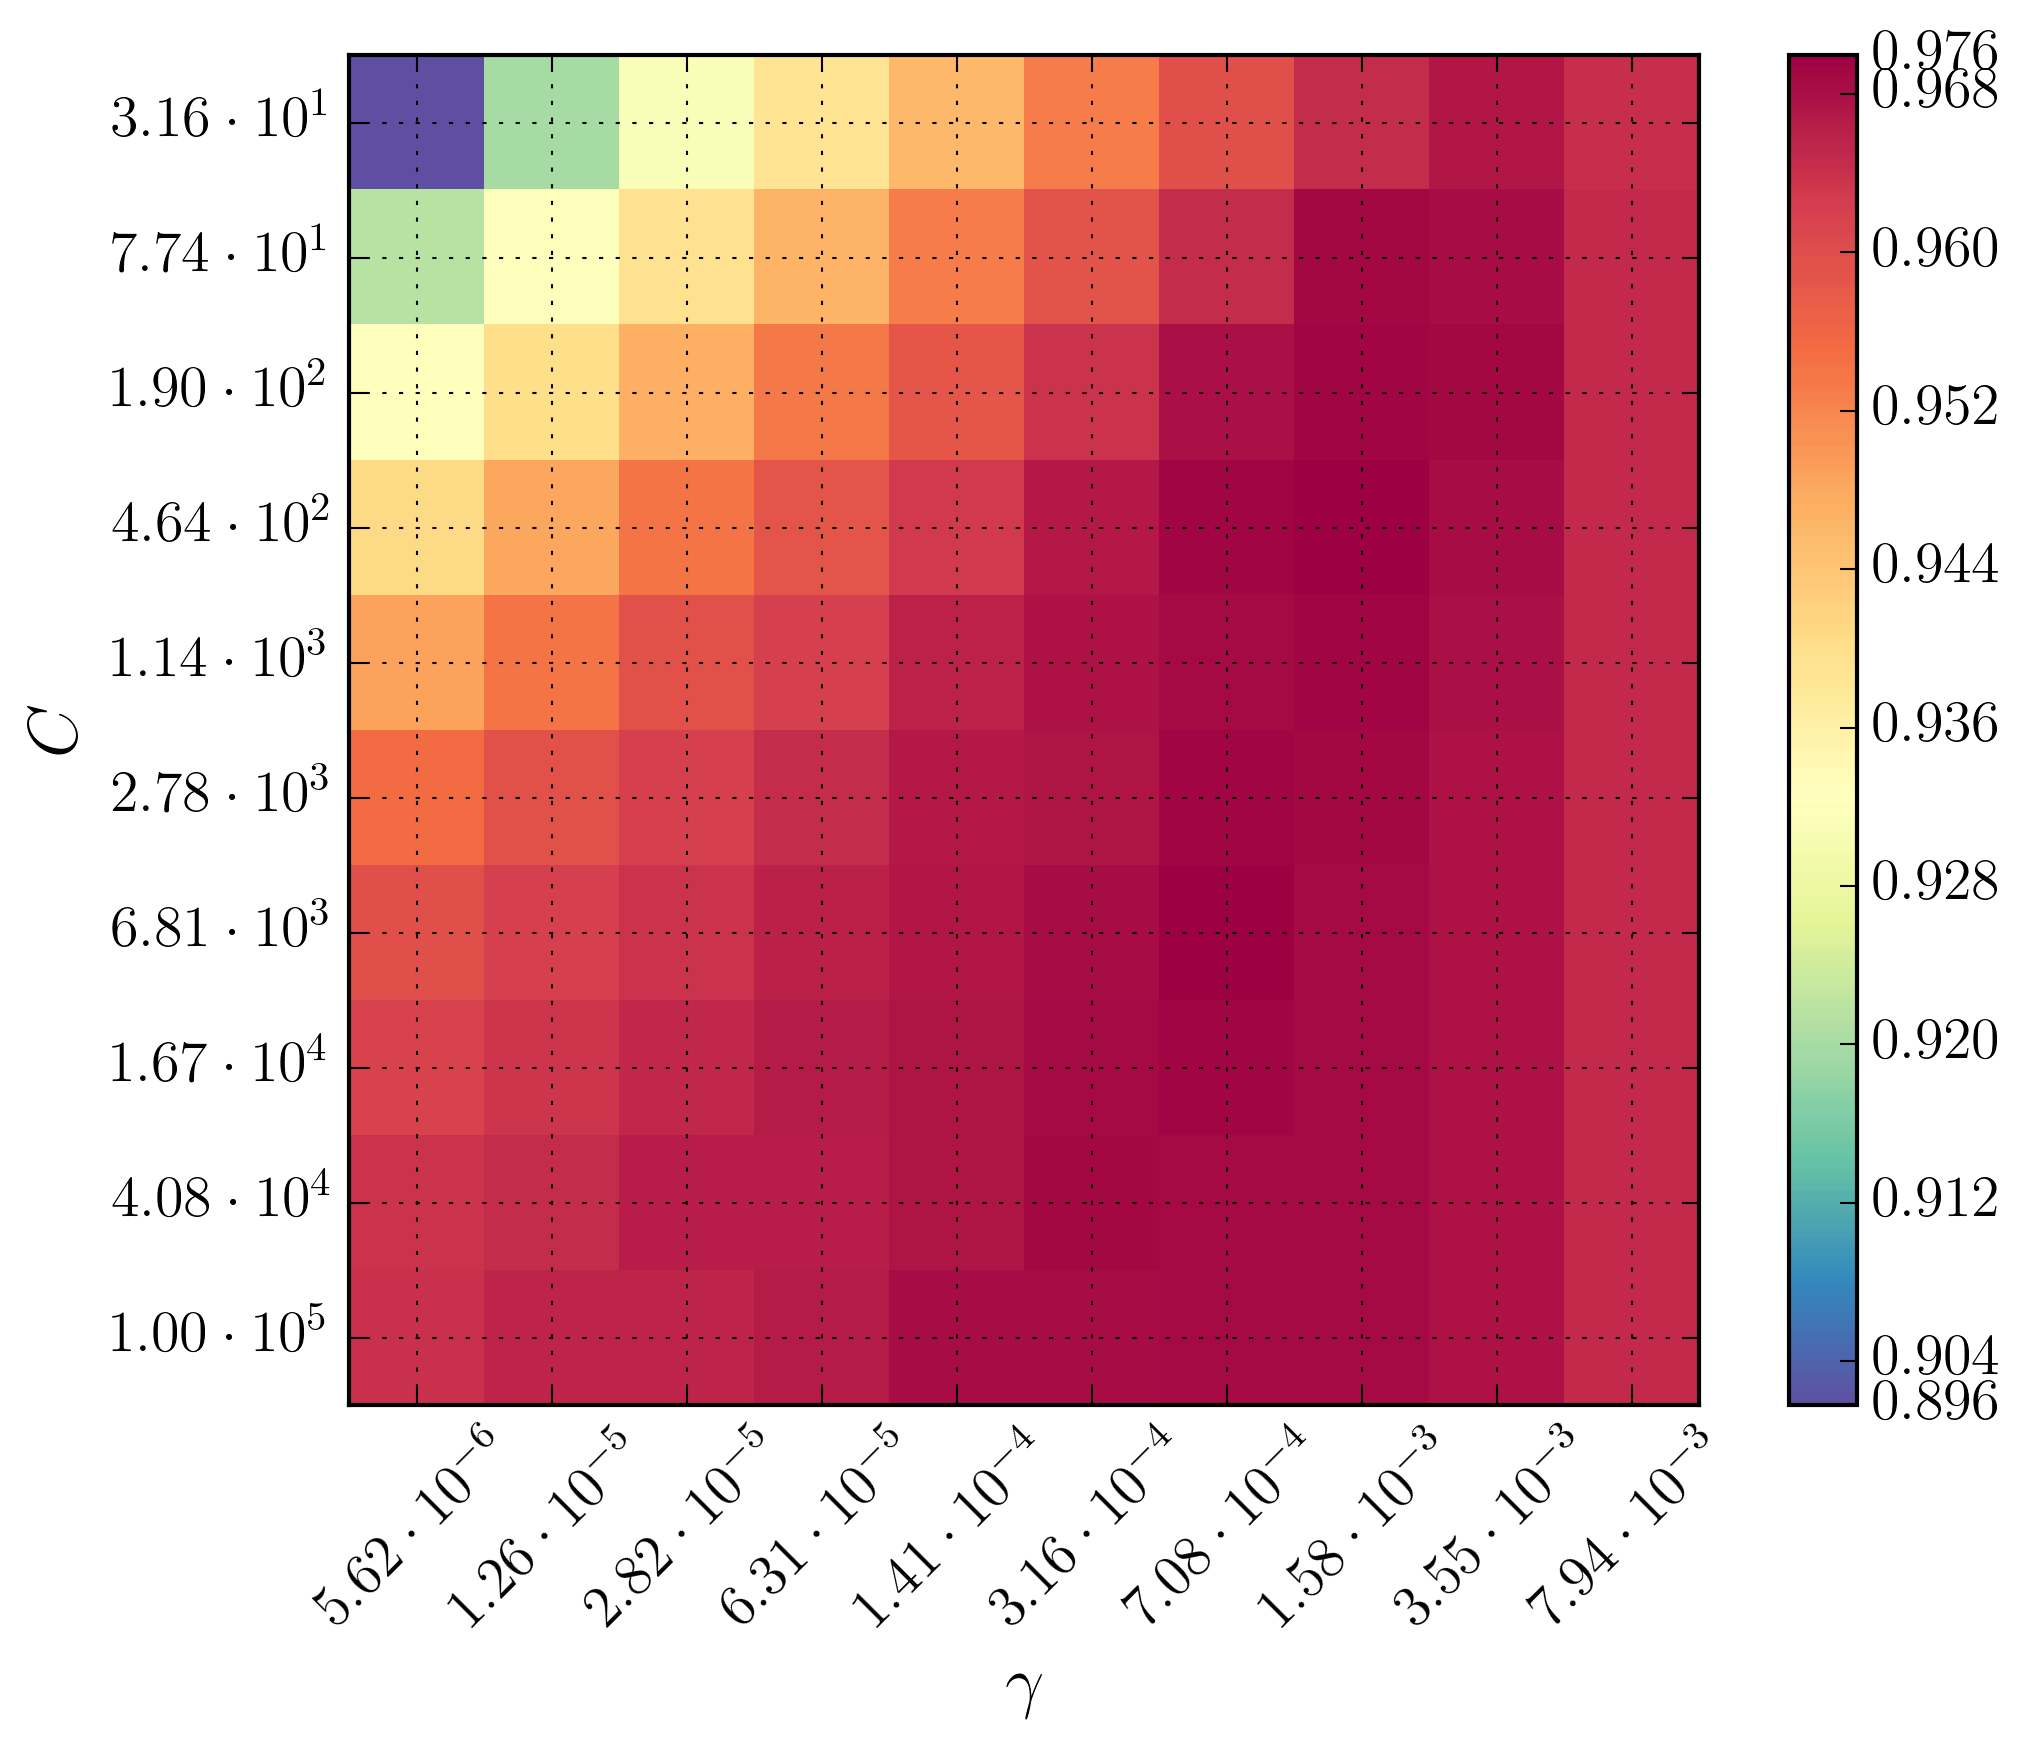
\includegraphics[width=0.49\textwidth,height=0.4\textwidth]{figures/gridsearch/svm/superclasses/svm-superclasses-03.png}}
\hfill
\subfigure{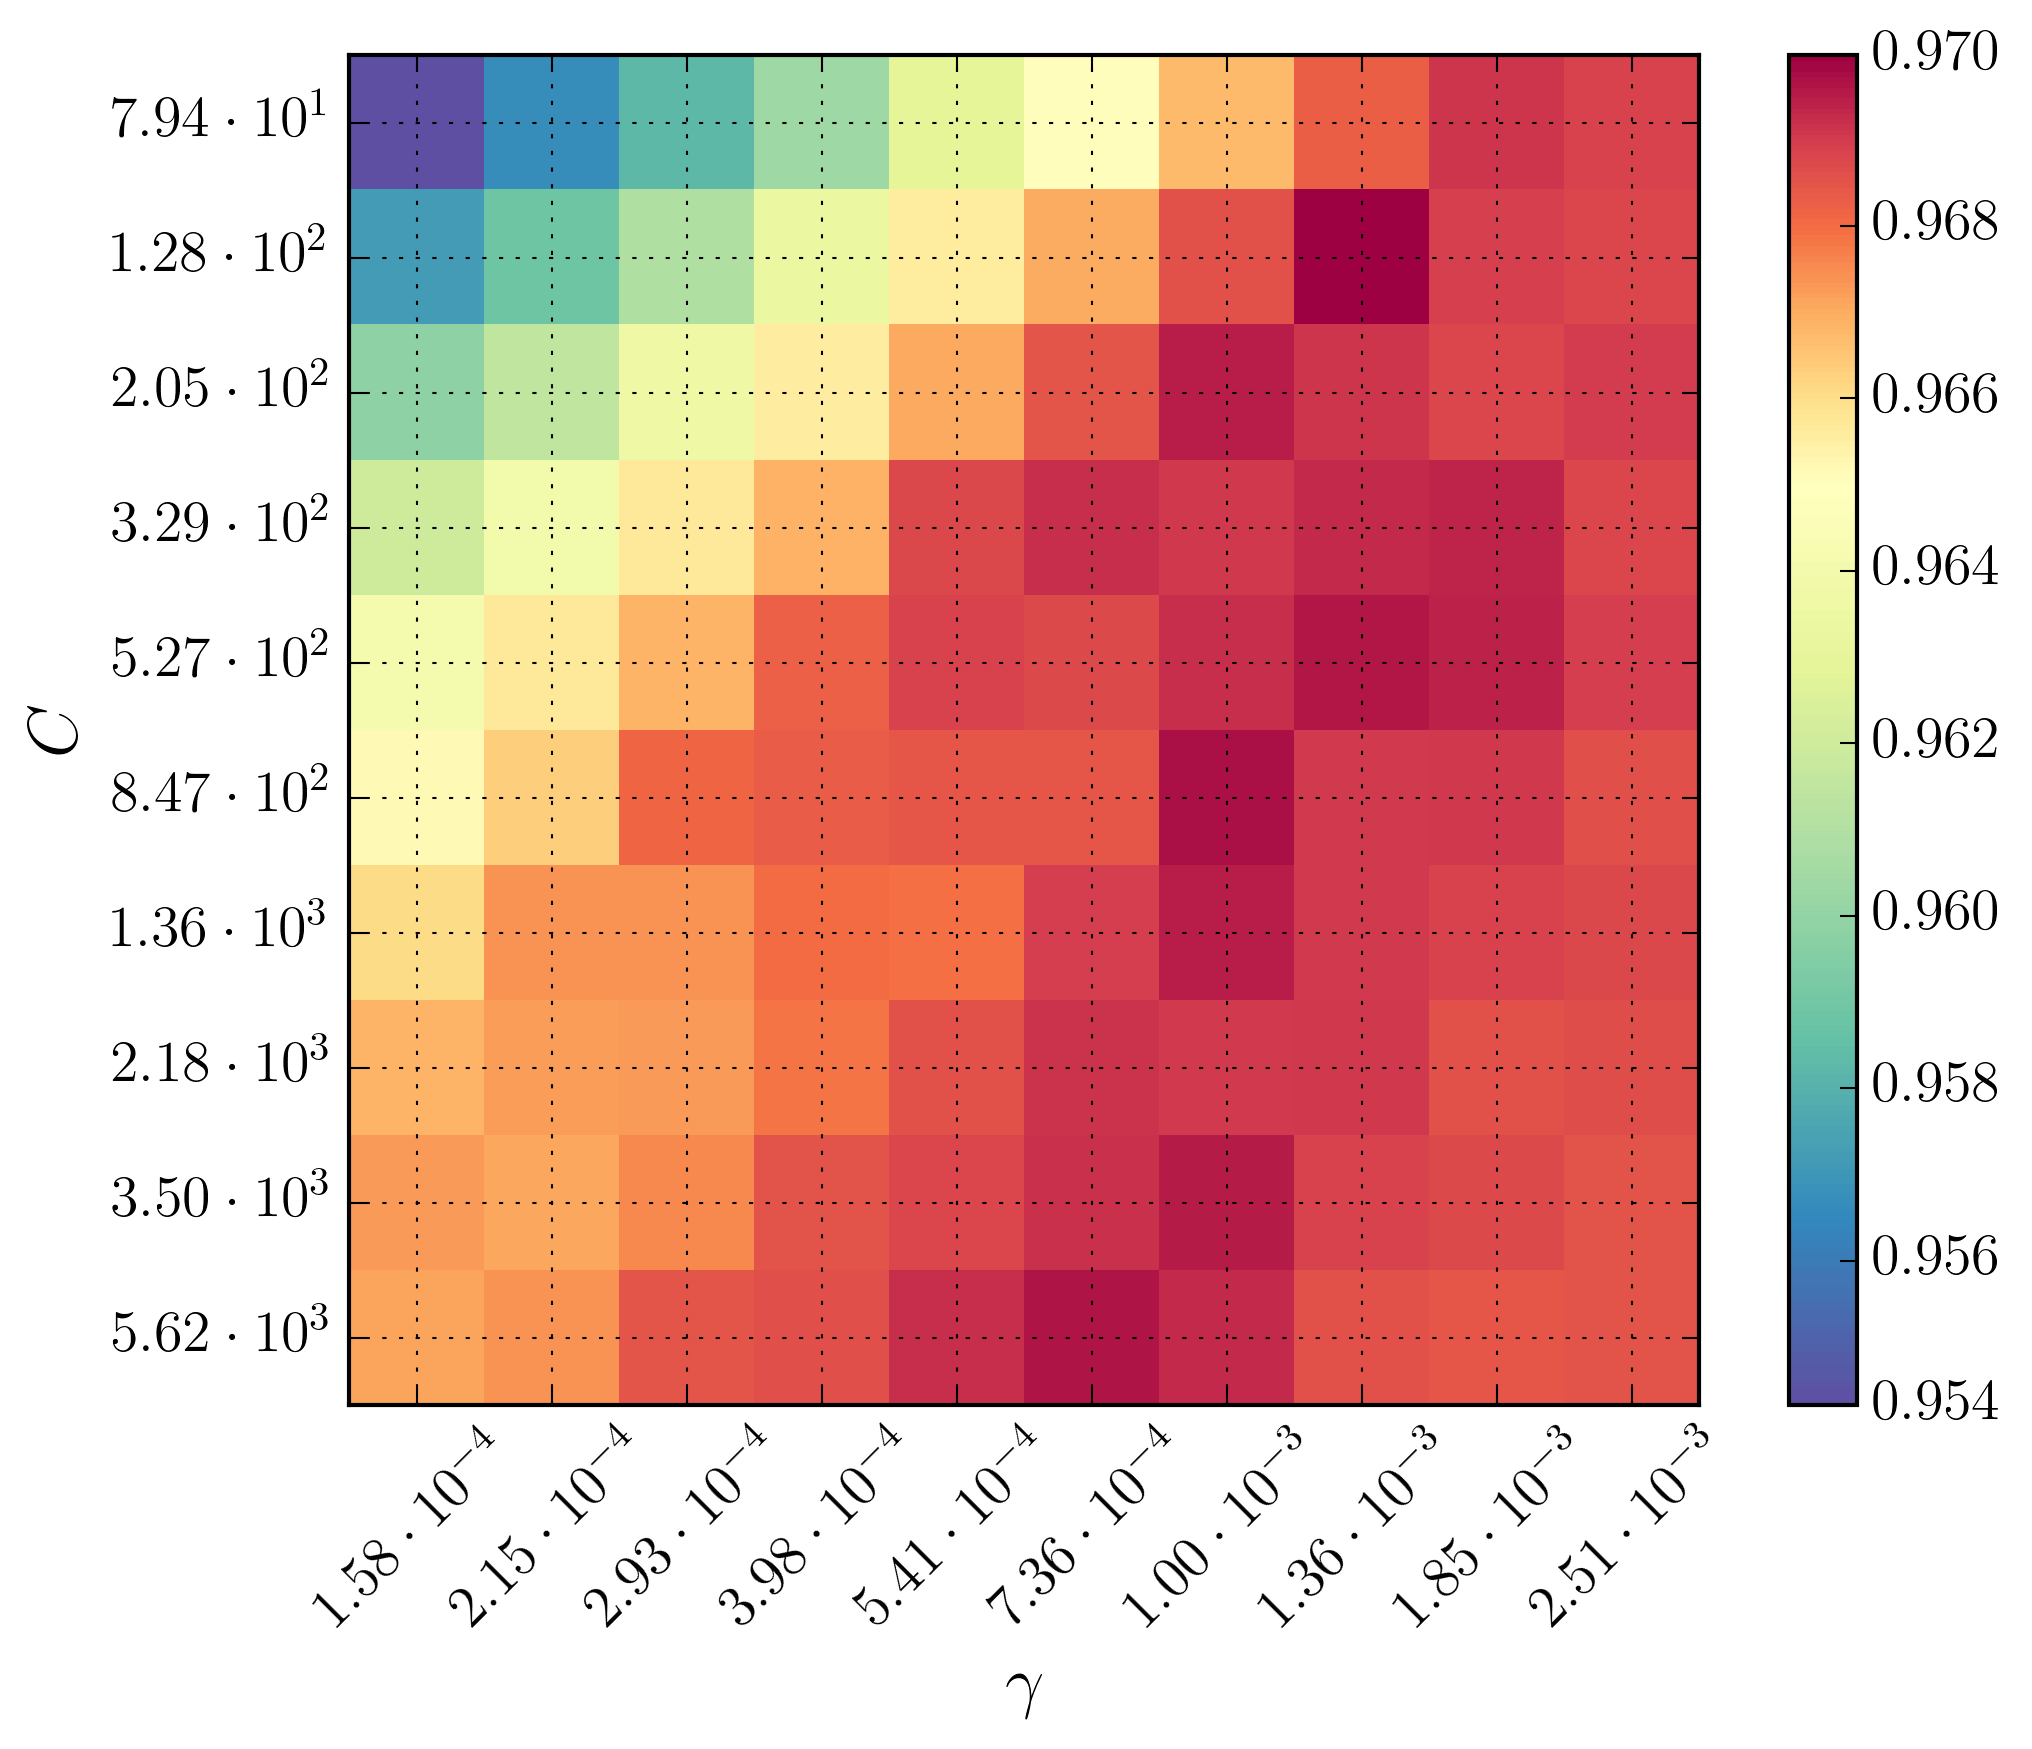
\includegraphics[width=0.51\textwidth,height=0.4\textwidth]{figures/gridsearch/svm/superclasses/svm-superclasses-04.png}}
\hfill
\subfigure{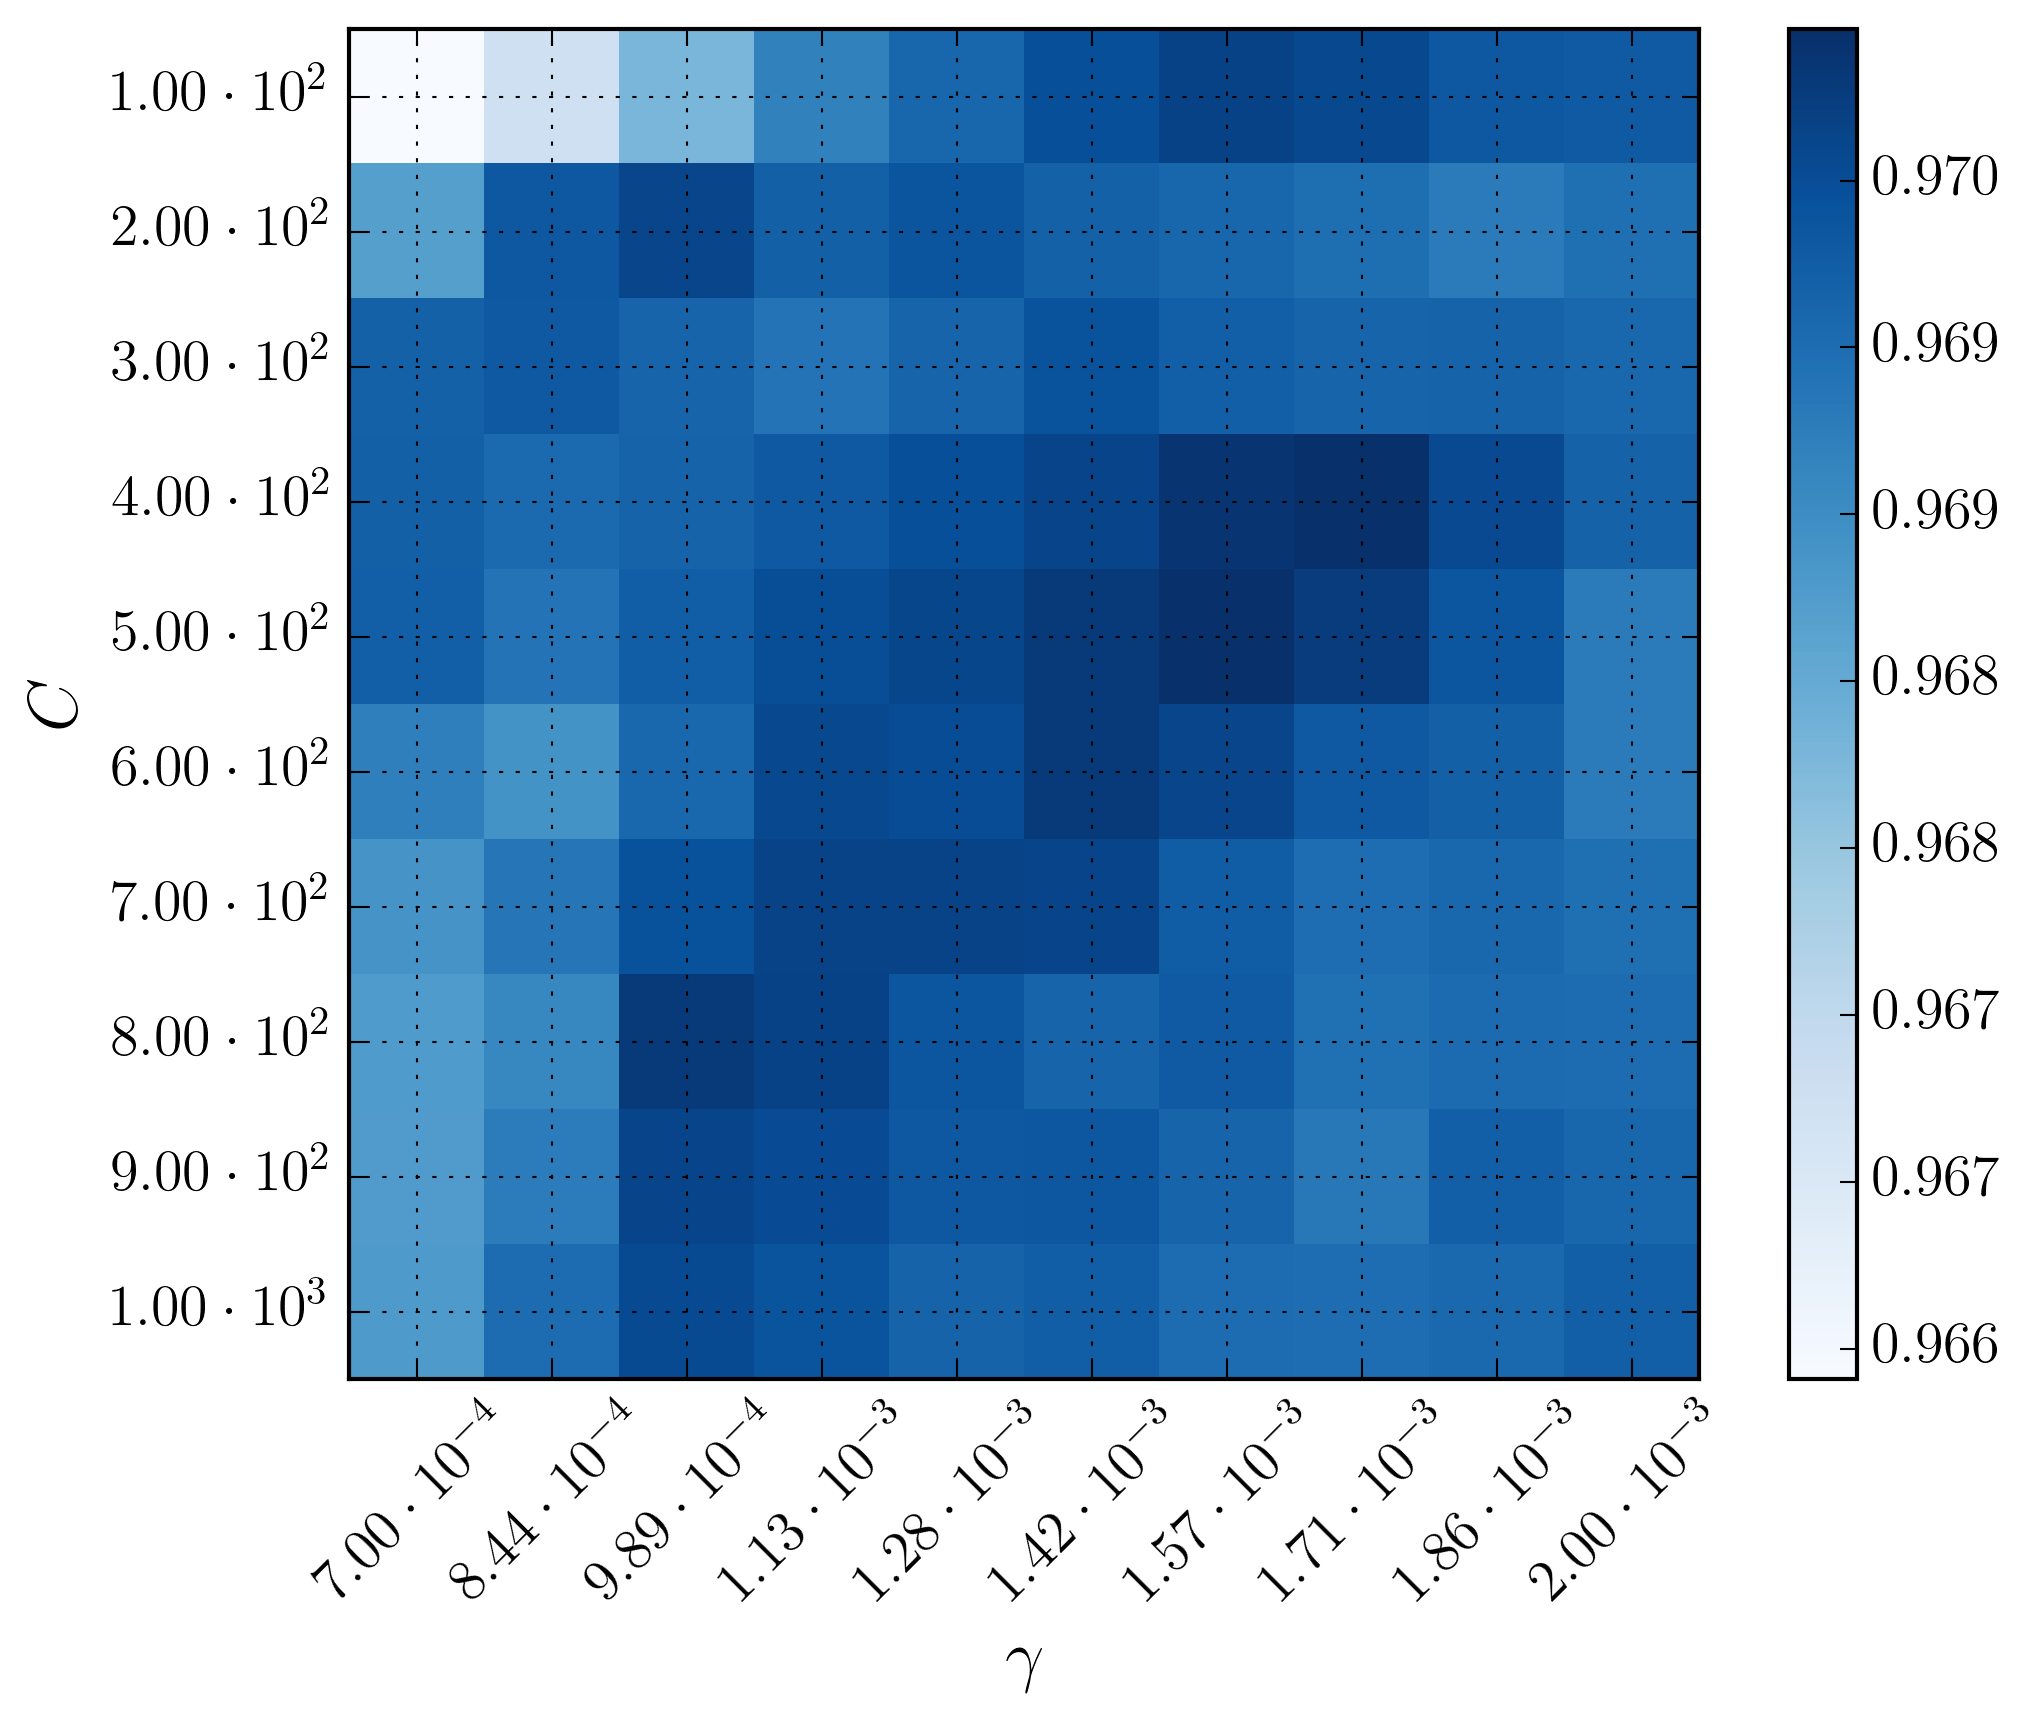
\includegraphics[width=0.49\textwidth,height=0.4\textwidth]{figures/gridsearch/svm/superclasses/svm-superclasses-05.png}}
\hfill
\subfigure{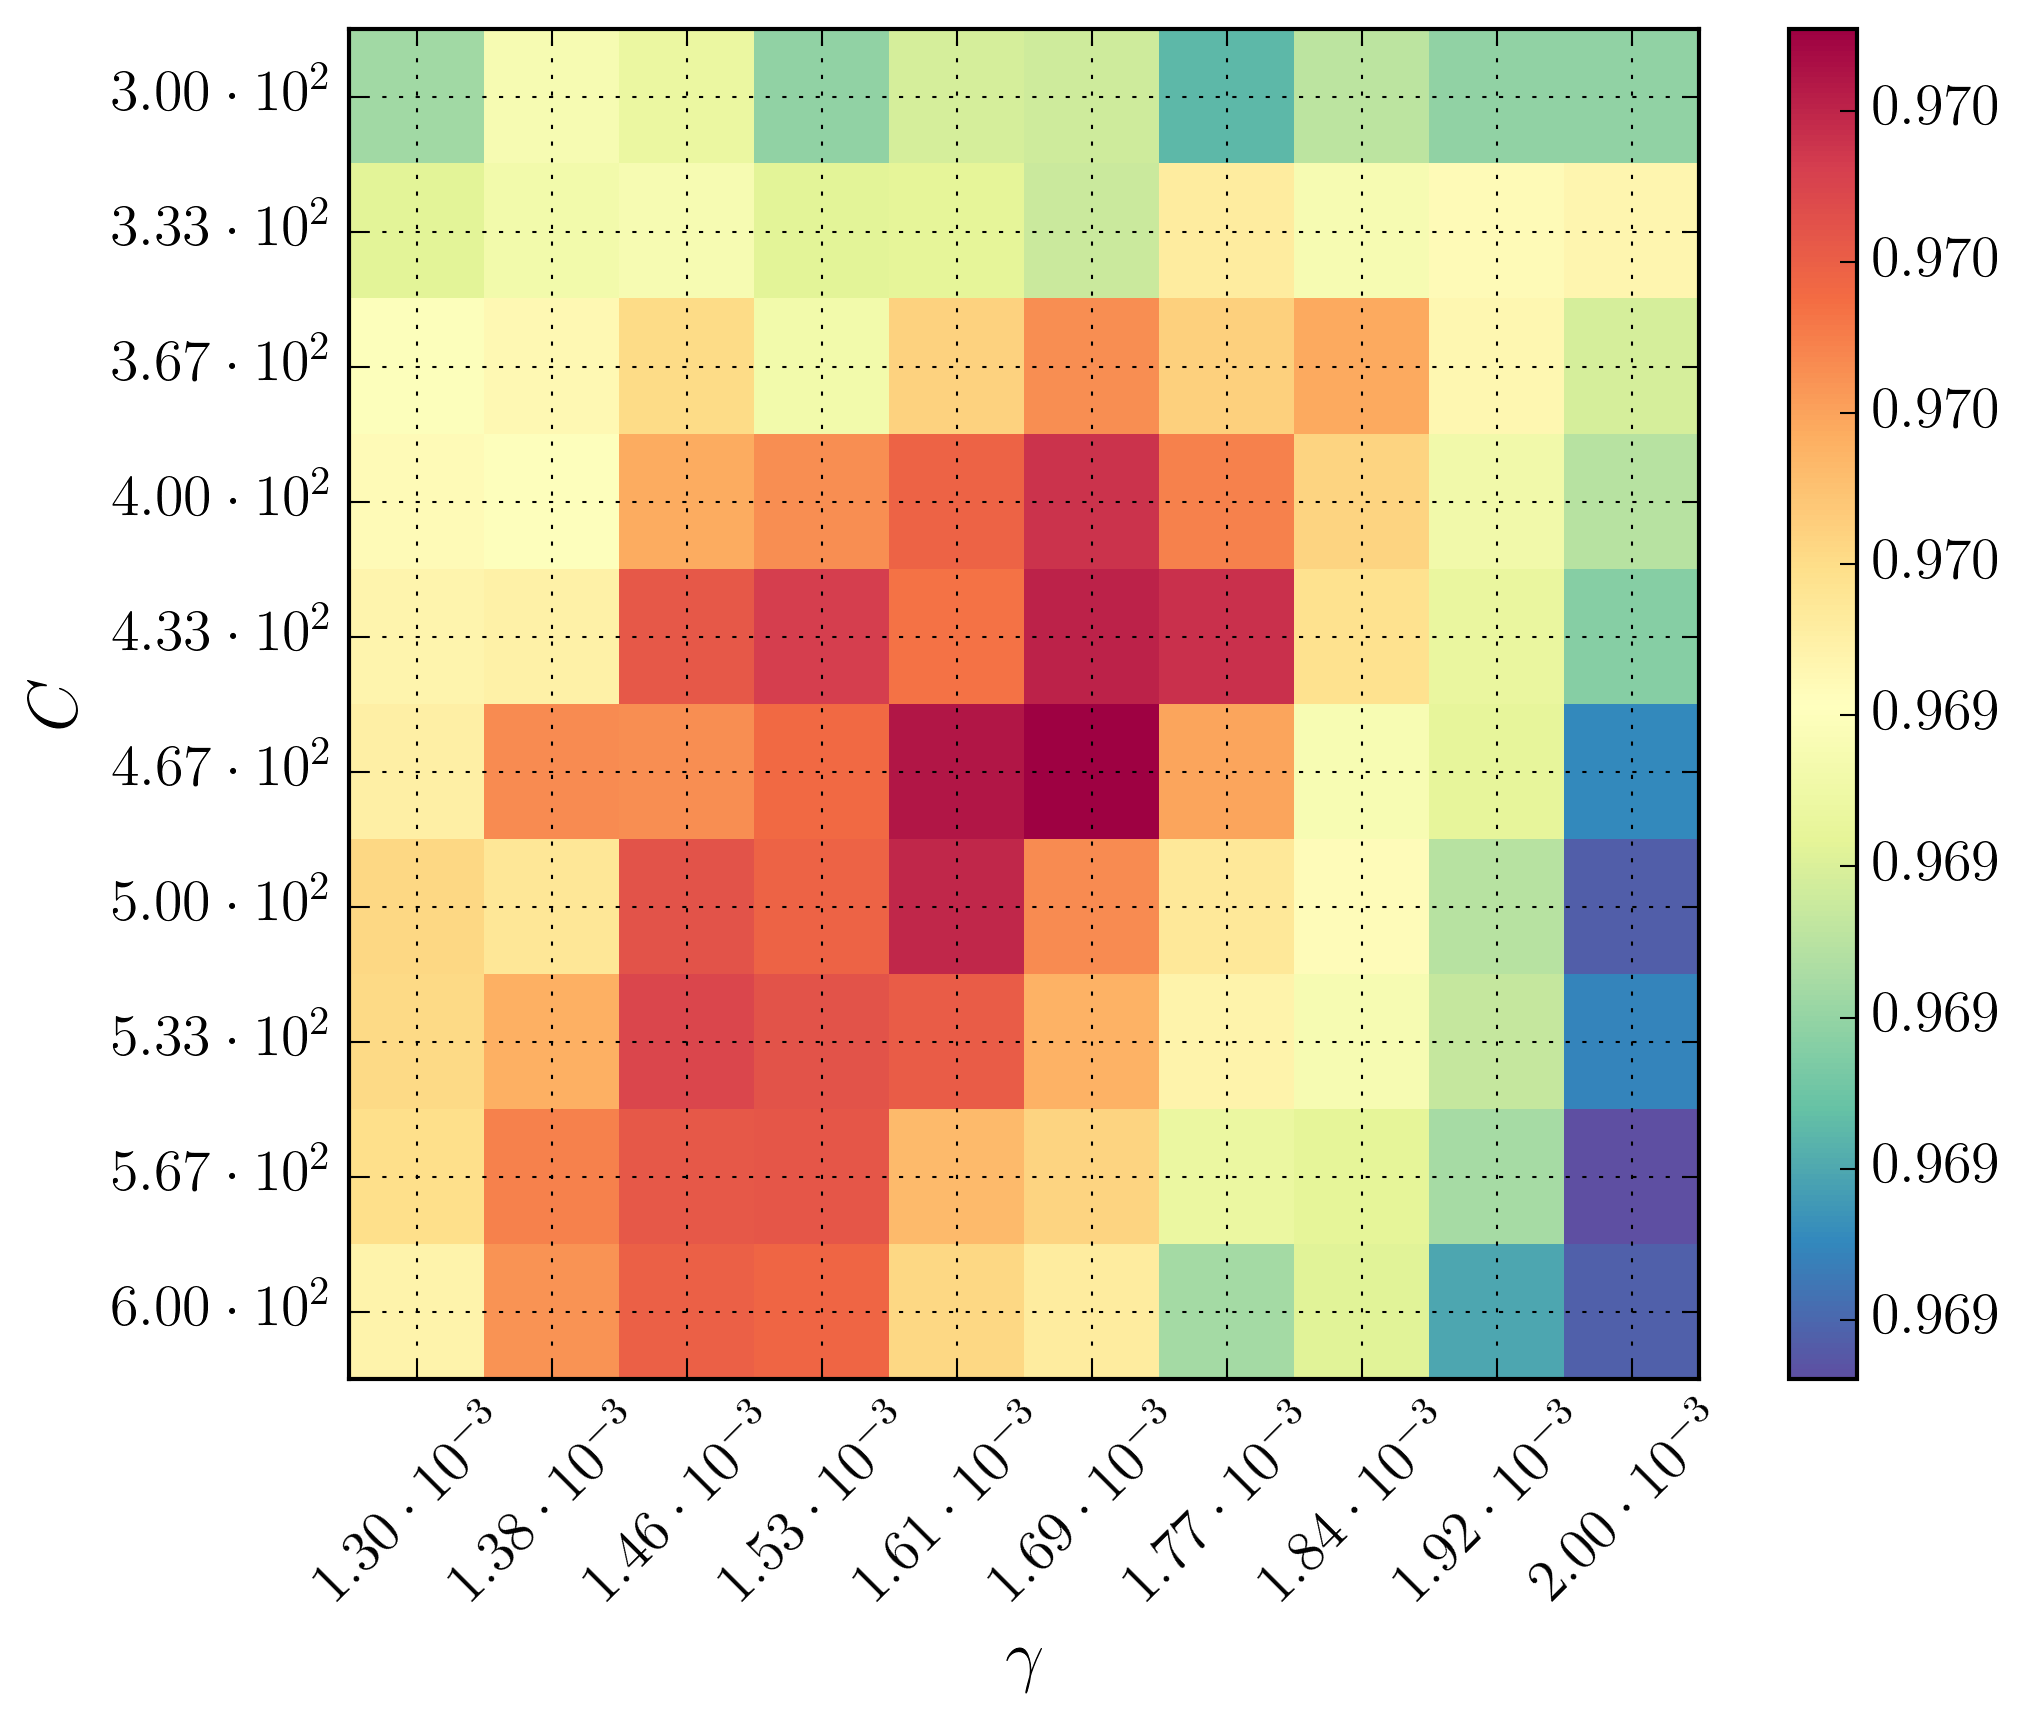
\includegraphics[width=0.51\textwidth,height=0.4\textwidth]{figures/gridsearch/svm/superclasses/svm-superclasses-06.png}}
\hfill
\caption[Hyperparameter optimization for the Support Vector Machine (SVM)]{This figure shows the average, weighted $F_1$ score on the $C$-$\gamma$-plane during the hyperparameter optimization for the Support Vector Machine. We start looking for global optima on a coarse grid with a wide range (upper left), and adjust the grid toward a finer stepwidth. At some point we find an optimum (lower right).}
\label{fig:gridsearch-svm-superclasses}
\end{figure}

We determine the optimal hyperparameters for the superclass classification to be $C = 4.67 \cdot 10^{2}$ and $\gamma = 1.69 \cdot 10^{-3}$.

% Hyperparameter optimization
% Add confusion matrix for main classes
% Add confusion matrix for subclasses

\renewcommand{\arraystretch}{1.5}
\resizebox{\textwidth}{!}{
\begin{tabular}{c|ccccccccc|c}
\toprule
%& \multicolumn{8 }{c}{Predicted class} & & \\
%\hline
                   & BV        & CEPH       & DSCT      & EB         & LPV         & NoneVar    & QSO       & RRL        & T2CEPH   & $\Sigma $ \\
\hline
BV                 & {\bfseries 762} &            &           &     12     &     1       &     19     &      1    &            &     1    &     796   \\
CEPH               &     2     & {\bfseries 2218} &           &     13     &     5       &     3      &           &     28     &    12    &    2281   \\
DSCT               &           &      5     & {\bfseries 453} &     8      &             &     17     &           &     28     &          &     511   \\
EB                 &    16     &      16    &     10    & {\bfseries 3336} &     50      &     54     &      5    &     46     &     5    &    3538   \\
LPV                &     5     &      5     &           &     46     & {\bfseries 15884} &     51     &      2    &     2      &          &   15995   \\
NoneVar            &    15     &      1     &     14    &     48     &     65      & {\bfseries 4621} &      24   &     3      &          &    4791   \\
QSO                &     2     &      1     &           &     1      &      1      &     30     & {\bfseries 144} &     1      &          &     180   \\
RRL                &           &      27    &     34    &     60     &      4      &     7      &      0    & {\bfseries 4336} &     2    &    4470   \\
T2CEPH             &     1     &      23    &           &     16     &      6      &     1      &           &     11     & {\bfseries 63} &     121   \\
\bottomrule
Recall ($\%$)      &   95.73   &     97.24  &   88.65   &    94.29   &    99.31    &   96.45    &    80.00  &    97.00   &   52.07  &           \\
\hline
Precision ($\%$)   &   94.89   &     96.60  &   88.65   &    94.24   &    99.18    &   96.21    &    81.82  &    97.33   &   75.90  &           \\
\hline
$F_1$ score ($\%$) &   95.31   &     96.92  &   88.65   &    94.26   &    99.24    &   96.33    &    80.90  &    97.16   &   61.77  & 97.25 $\pm$ 0.25 \\
\bottomrule
\end{tabular}
%\caption{This table shows the confusion matrix for superclass classification on the EROS data set with $C = 4.67 \cdot 10^{2}$ and $\gamma = 1.69 \cdot 10^{-3}$. The columns show predicted labels, while rows show the true label.}
}

Furthermore, we also want the classifier to predict subclasses as well...

\begin{landscape}
\resizebox{22cm}{!}{
\begin{tabular}{c|C{1cm}C{1cm}C{1cm}C{1cm}C{1cm}C{1cm}C{1cm}C{1cm}C{1cm}C{1cm}C{1cm}C{1cm}C{1cm}C{1cm}C{1cm}C{1cm}C{1cm}C{1cm}C{1cm}C{1cm}|c}
\toprule
 &   1O &      EC &        ED &   ED ESD &      ESD &        F &   Mira AGB C &   Mira AGB O &         N &   OSARG AGB C &   OSARG AGB O &   OSARG RGB C &   OSARG RGB O &   Other &      RRab &      RRc &     RRd &     RRe &   SRV AGB C &   SRV AGB O & $\Sigma$ \\
\midrule
1O                 & \bfseries 720      &   5     &    1      &          &   5      &   53     &              &              &   14      &               &               &               &        1      &  26     &    9      &   9      &  1      &         &             &             & .... \\
EC                 &   6      & \bfseries 268     &    5      &   3      &  95      &    2     &              &              &    7      &        2      &               &               &       12      &  20     &   13      &   6      &  1      &  4      &             &      1      & .... \\
ED                 &   3      &  22     & \bfseries 1224      & 101      & 255      &          &              &              &   18      &        1      &               &               &        1      &  17     &    1      &          &  1      &         &             &             & .... \\
ED ESD             &          &   3     &   87      &  \bfseries 10      &  24      &          &              &              &   20      &               &               &               &               &   2     &           &          &         &         &             &             & .... \\
ESD                &   4      & 138     &  197      &  26      & \bfseries 707      &    1     &              &              &   20      &               &        1      &               &       12      &  35     &    2      &   5      &  1      &  1      &             &             & .... \\
F                  & 120      &   1     &           &          &   1      & \bfseries 1132     &       1      &              &    5      &               &        1      &               &               &   8     &    6      &          &         &         &             &             & .... \\
Mira AGB C         &          &         &           &          &          &          &     \bfseries 679      &      14      &    9      &               &               &               &        1      &         &           &          &         &         &     50      &      1      & .... \\
Mira AGB O         &          &         &           &          &          &          &      24      &     \bfseries 271      &    1      &               &               &               &               &         &           &          &         &         &      3      &     30      & .... \\
N                  &  34      &  22     &   37      &  19      &  31      &    8     &       2      &              & \bfseries 6068      &       28      &       34      &        2      &       17      &  22     &   18      &  22      &  3      & 28      &      1      &      3      & .... \\
OSARG AGB C        &          &         &           &          &          &          &              &              &   27      &      \bfseries 963      &      199      &        6      &       15      &         &           &          &         &         &    192      &     14      & .... \\
OSARG AGB O        &          &   2     &           &          &   4      &          &              &              &   33      &      379      &     \bfseries 2360      &        5      &      183      &   3     &           &          &         &         &     15      &    384      & .... \\
OSARG RGB C        &          &         &           &          &          &          &              &              &    8      &        7      &       14      &        \bfseries 3      &       17      &         &           &          &         &         &      7      &      1      & .... \\
OSARG RGB O        &          &  10     &    1      &          &   9      &          &       1      &              &   18      &       28      &      148      &       19      &     \bfseries 1708      &   3     &    1      &          &         &         &      1      &     99      & .... \\
Other              &  31      &  26     &   24      &   3      &  35      &    6     &              &              &   26      &        2      &        1      &               &       10      & \bfseries 135     &   11      &   2      &  1      &  1      &             &      1      & .... \\
RRab               &   9      &  34     &    1      &   2      &  14      &   10     &              &              &   18      &               &        3      &               &               &  19     & \bfseries 3193      &  70      & 57      &  4      &             &             & .... \\
RRc                &   4      &  14     &    3      &          &   6      &          &              &              &   19      &               &               &               &               &   5     &   40      & \bfseries 570      & 22      & 31      &             &             & .... \\
RRd                &          &   3     &    2      &          &          &          &              &              &    3      &               &               &               &               &   1     &   44      &  43      & \bfseries 82      &  1      &             &             & .... \\
RRe                &   1      &   6     &           &   1      &   2      &          &              &              &   22      &               &               &               &               &   1     &    4      &  53      &  5      & \bfseries 48      &             &             & .... \\
RV AGB C           &          &         &           &          &          &          &      93      &       4      &    9      &      292      &       19      &        2      &        5      &         &           &          &         &         &   \bfseries 3298      &     97      & .... \\
RV AGB O           &   1      &   2     &           &          &          &          &       6      &      80      &   11      &       55      &      329      &       11      &      130      &   1     &           &          &         &         &    110      &   \bfseries 3470      & .... \\
\bottomrule
Recall ($\%$)      &   85.31  &   60.22 &    74.45  &   6.85   &   61.48  &    88.78 &  90.05       &      82.37   &   94.83   &        68.01  &      70.07    &        5.26   &      83.48    &   42.86 &    92.98  &  79.83   &  45.81  &  33.57  &    86.36    &  82.50  &        \\
\hline
Precision ($\%$)   &   77.17  &   48.20 &    77.37  &   6.06   &   59.51  &    93.40  &       84.24  &      73.44   &   95.47   &        54.81  &      75.91    &        6.25   &      80.87    &   45.30 &    95.54  &  73.08   &  47.13  &  40.68  &    89.69    &   84.61 &        \\
\hline
$F_1$ score ($\%$) &   .....  &   .... &    ....  &   ....   &  ....  &    ....  &       .... &     ....  &   ....   &        ....   &      ....     &       ....   &      ....     &   ....  &   ....  &  ....    &  ....   &  ....   &   ....    &   .... & $82.79 \pm 0.63$\\
\bottomrule
\end{tabular}
}
\end{landscape}

\section{Performance of the Random Forest Classifier}

The second classifier to evaluate is the Random Forest classifier. Once again, for optimal classification performance, we have to optimize the model's hyperparameters $t$, the number of trees in the forest, and $m$, the maximum number of features to consider at each split. The results of the $5$-fold cross--validation grid search (superclasses), optimized for the average $F_1$-score, weighted by the number of observations per class, shown in figure \ref{fig:gridsearch-rf-superclasses}.

\begin{figure}[H]
\subfigure{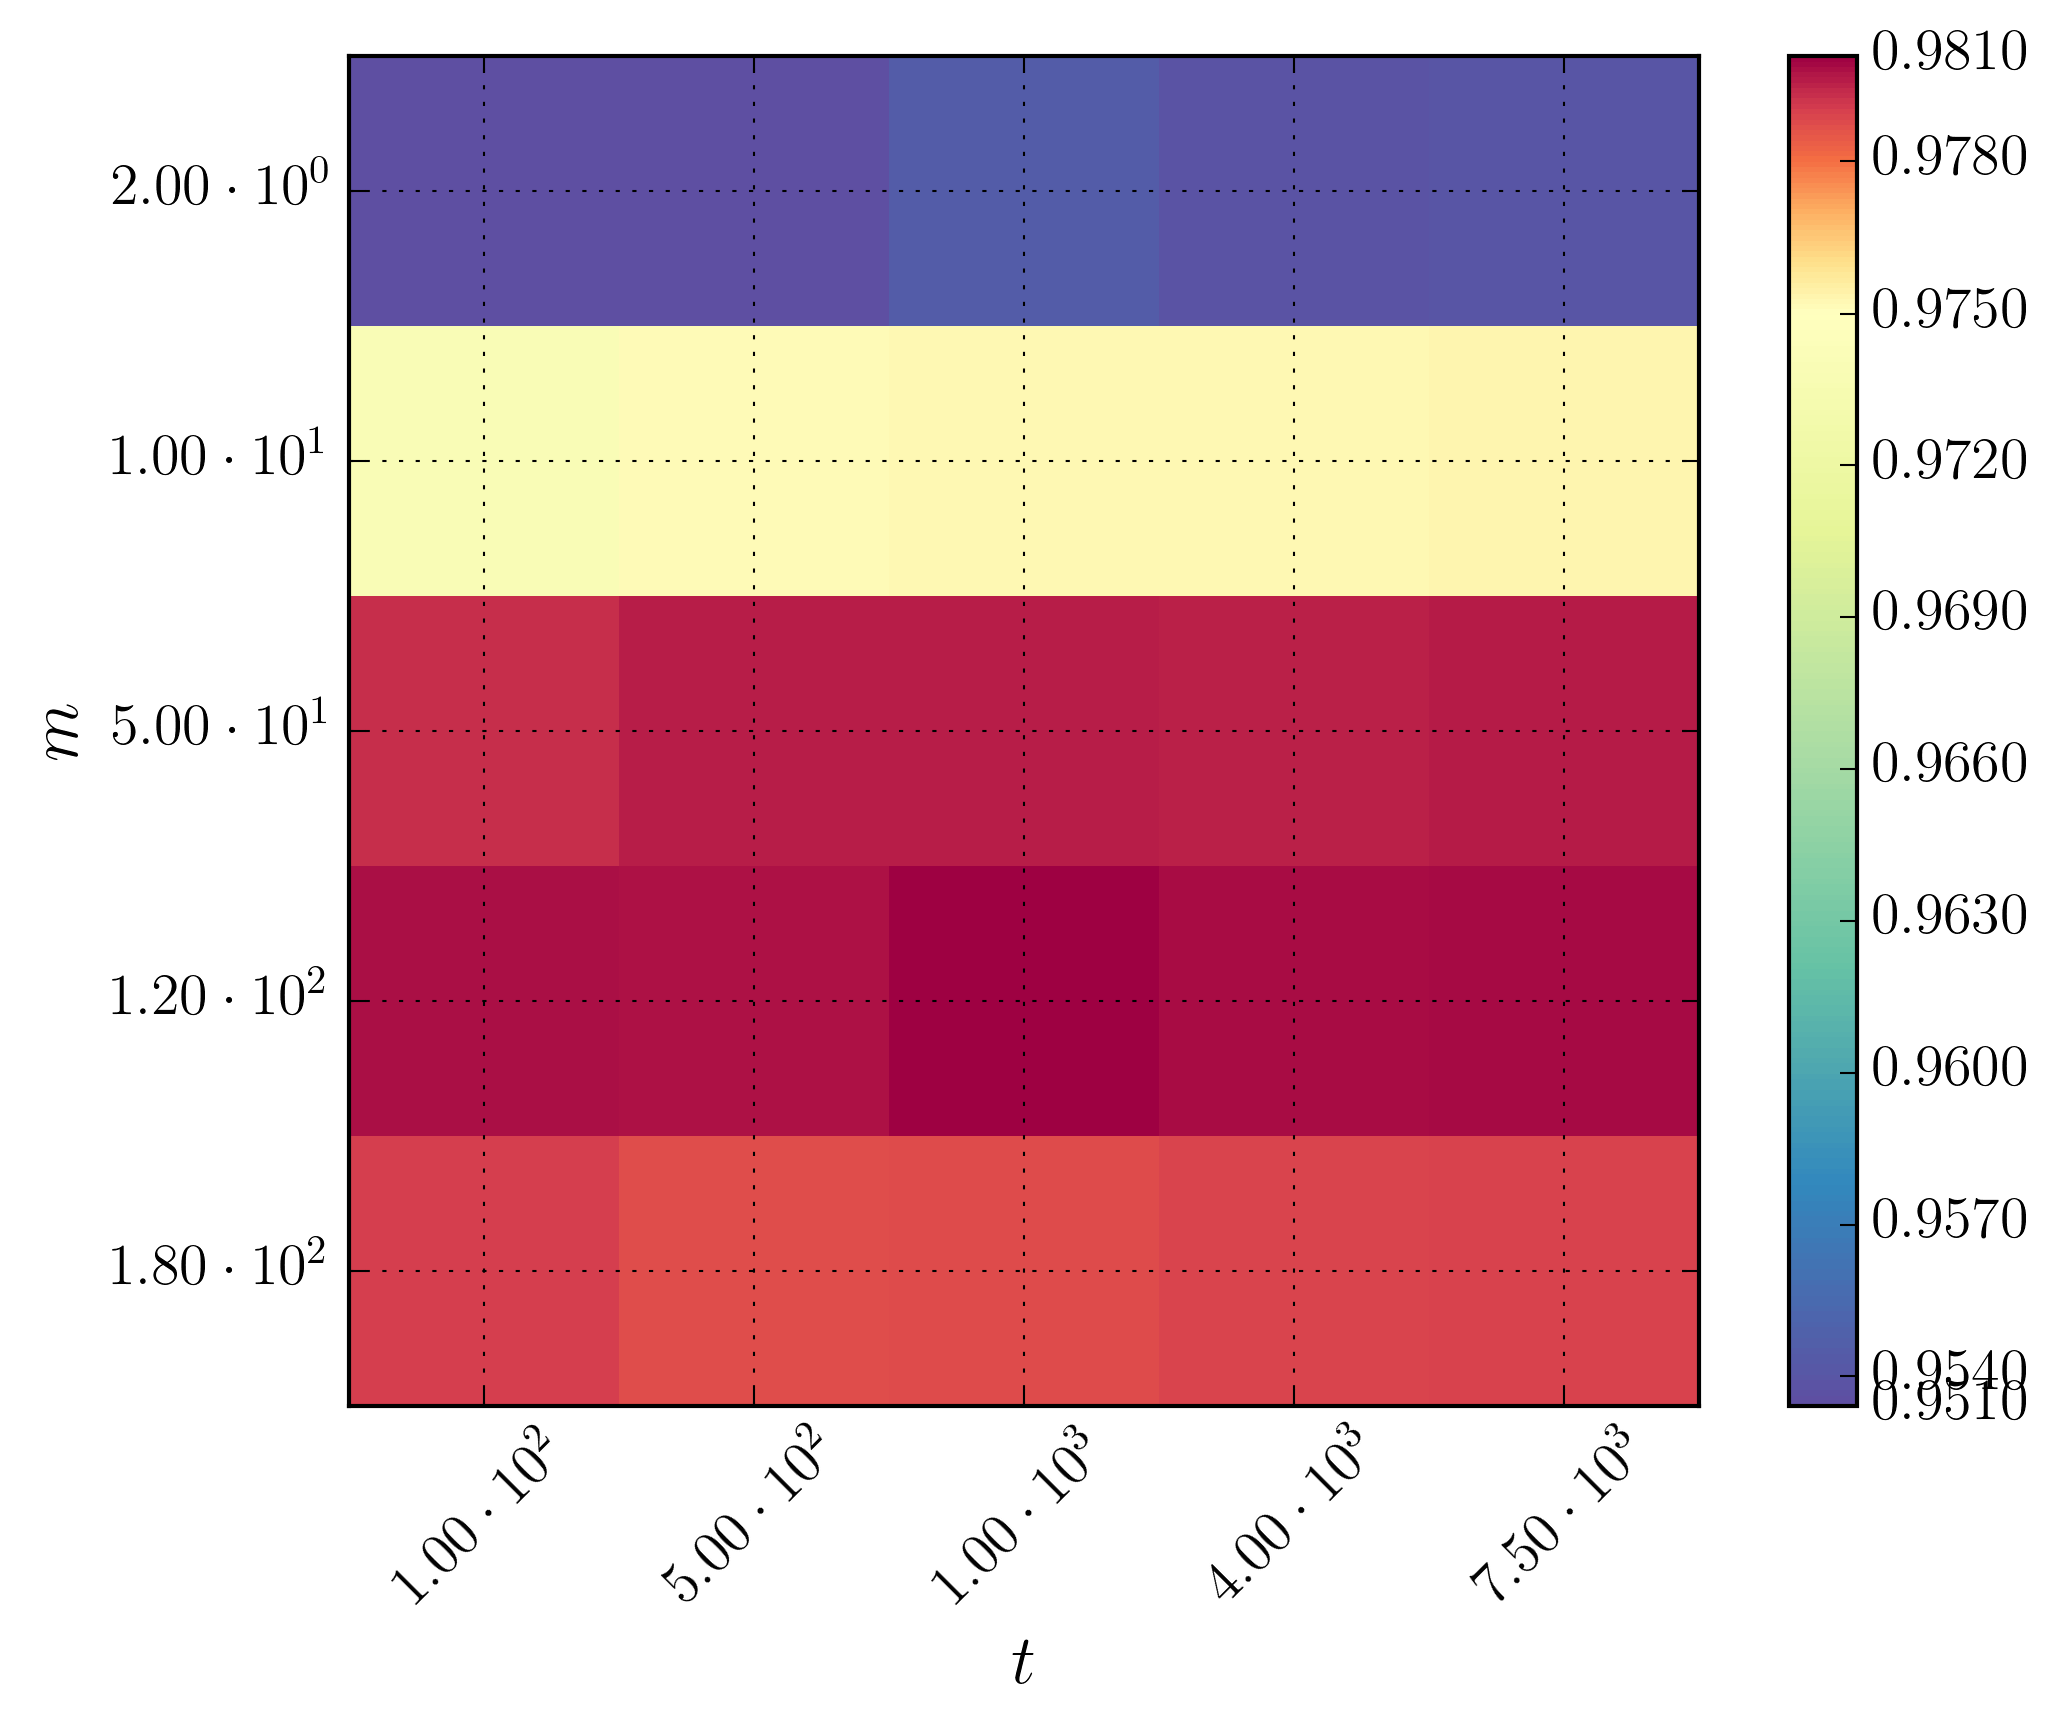
\includegraphics[width=0.49\textwidth,height=0.4\textwidth]{figures/gridsearch/rf/superclasses/rf-superclasses-01.png}}
\hfill
\subfigure{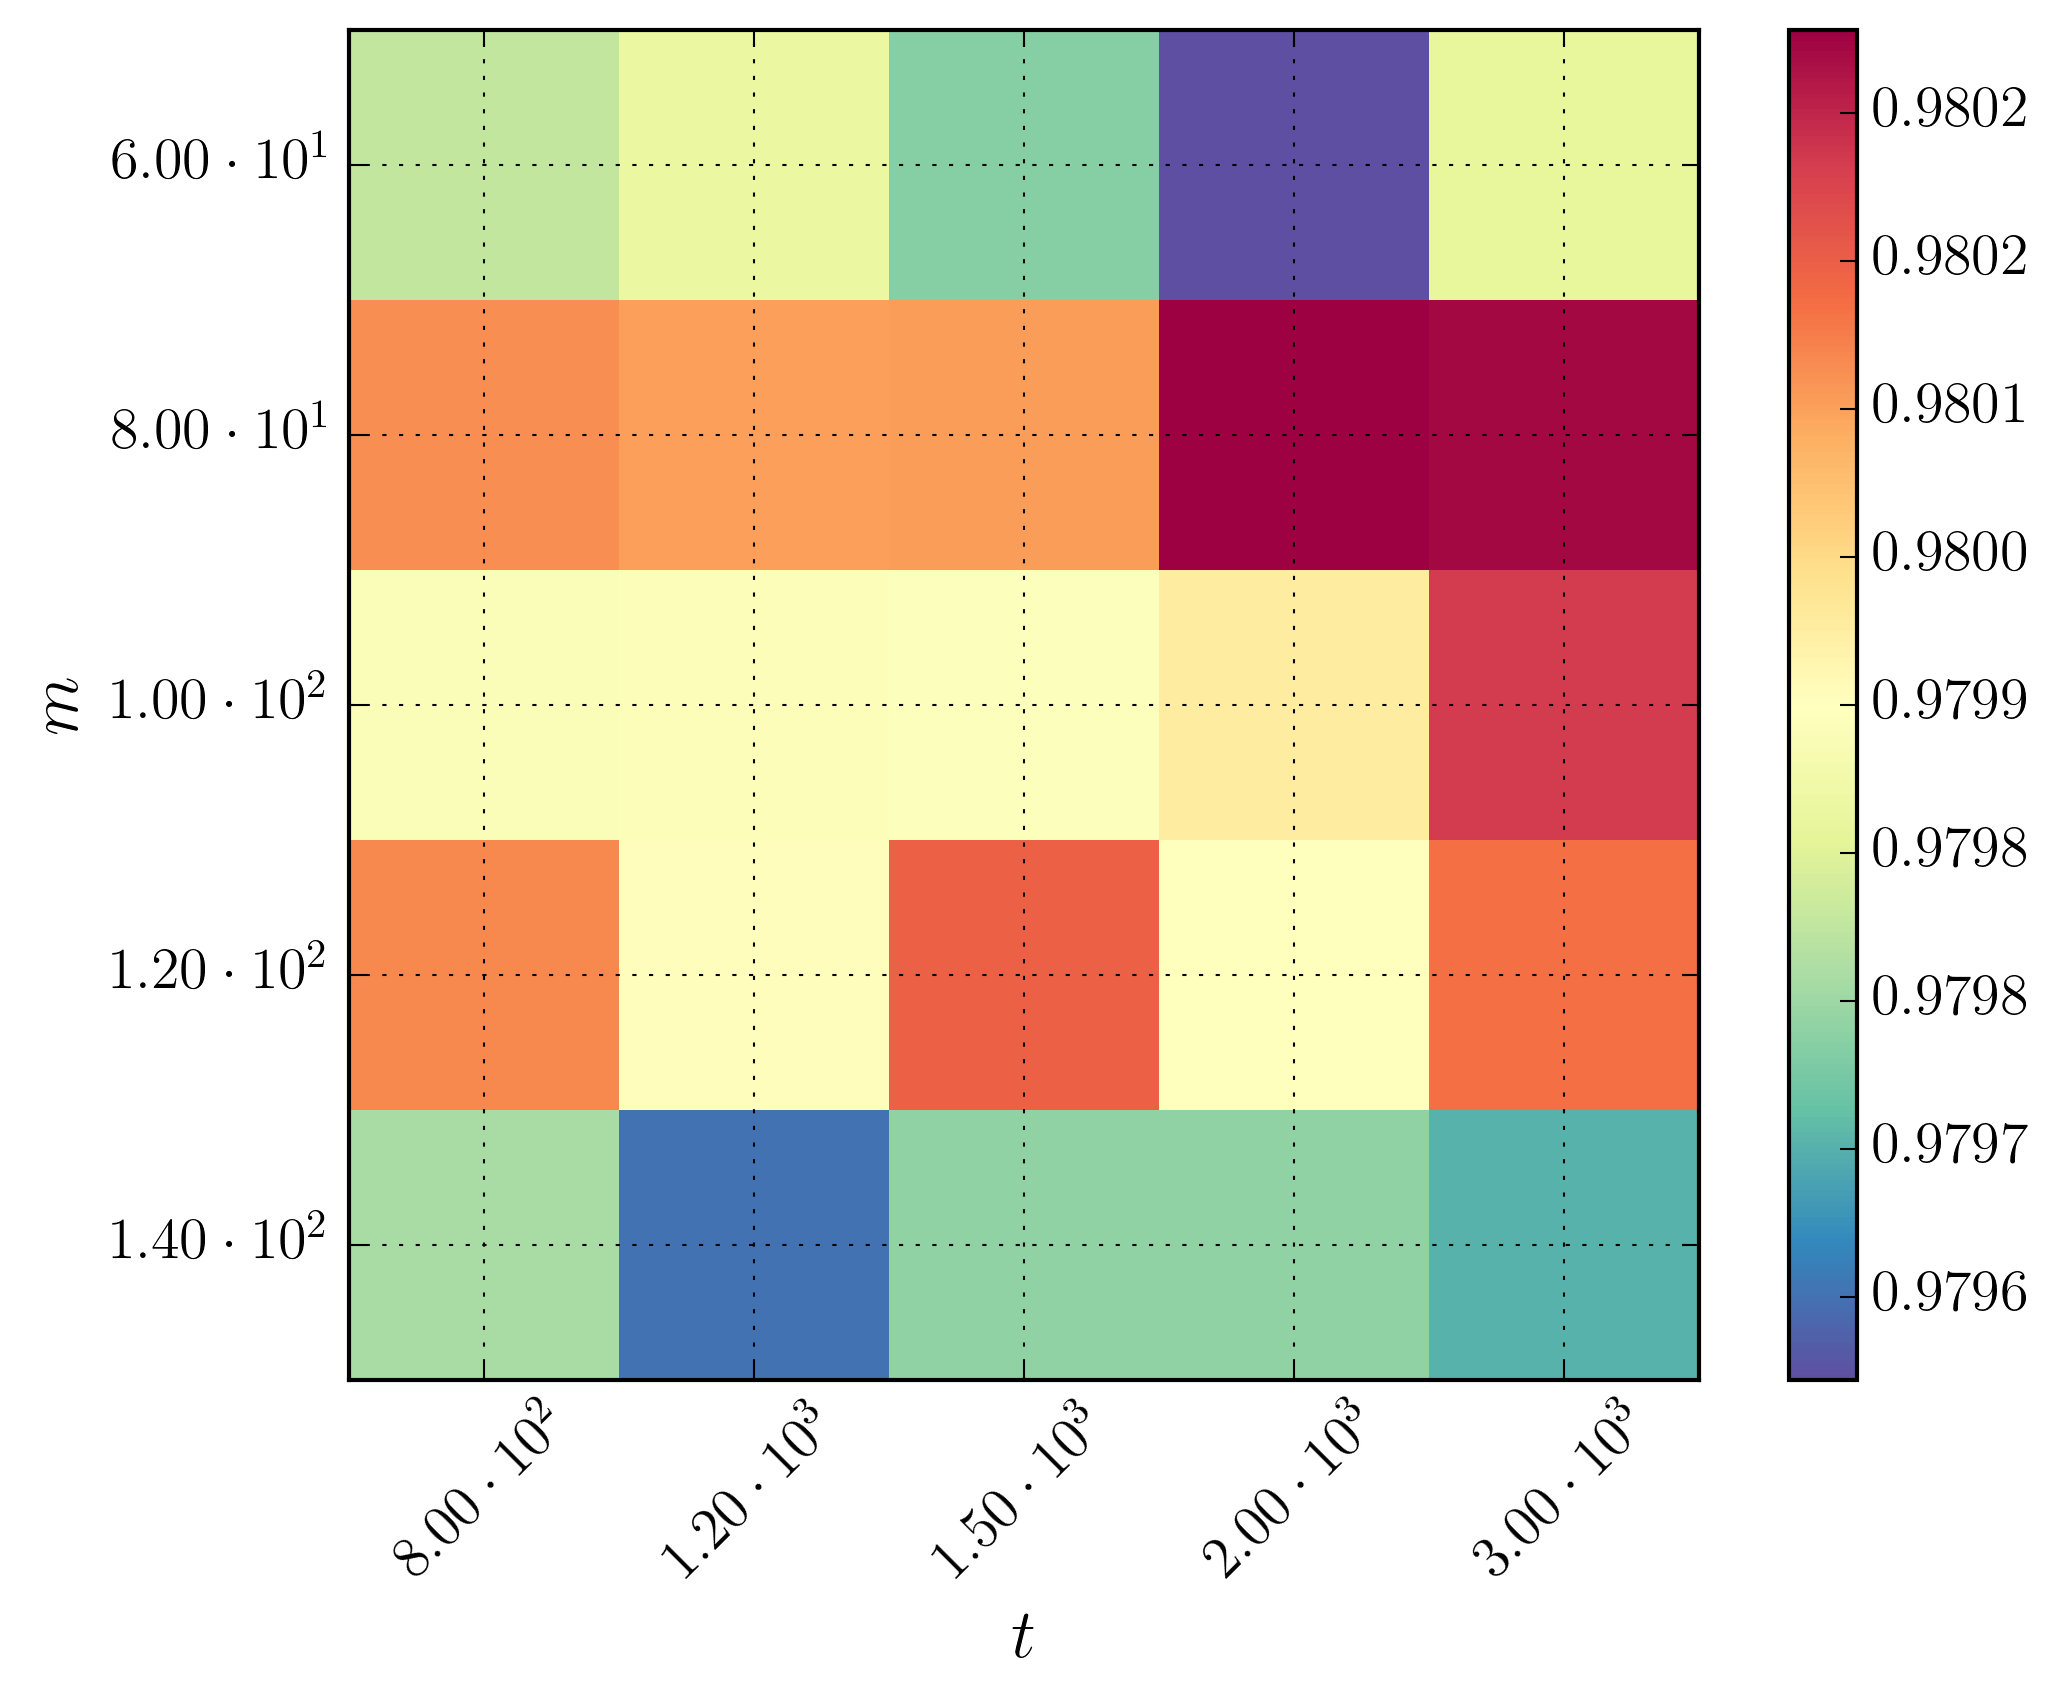
\includegraphics[width=0.51\textwidth,height=0.4\textwidth]{figures/gridsearch/rf/superclasses/rf-superclasses-02.png}}
\hfill
\subfigure{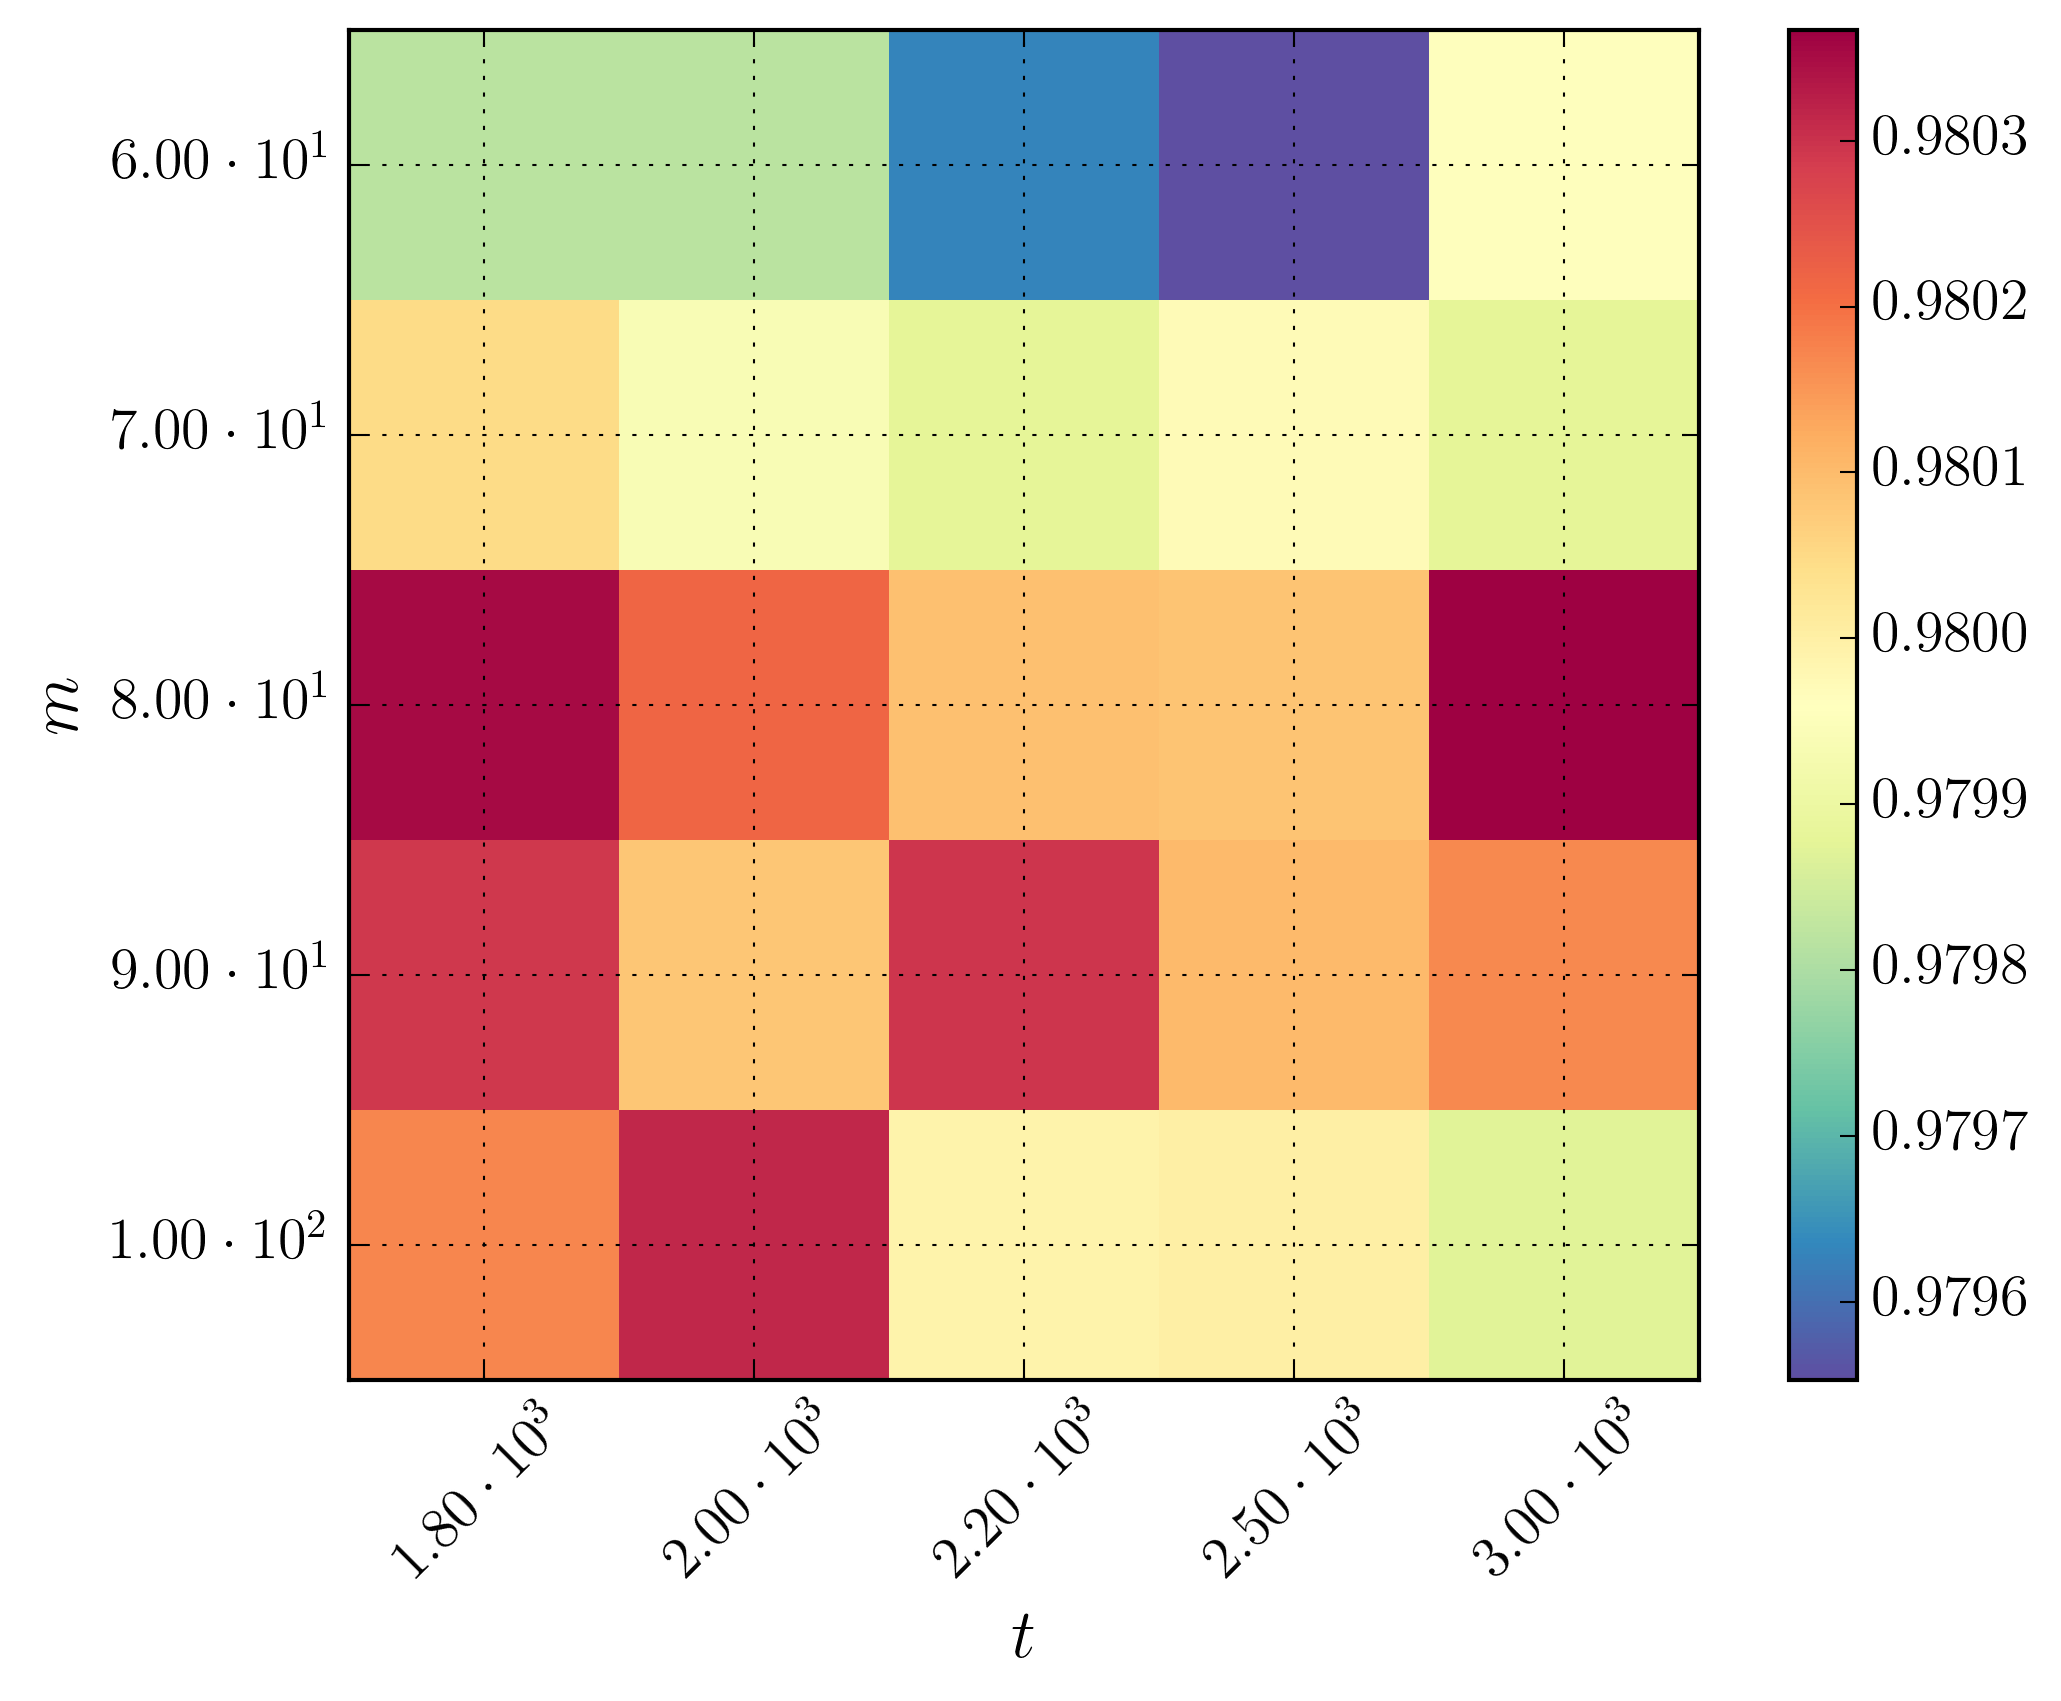
\includegraphics[width=0.49\textwidth,height=0.4\textwidth]{figures/gridsearch/rf/superclasses/rf-superclasses-03.png}}
\hfill
\subfigure{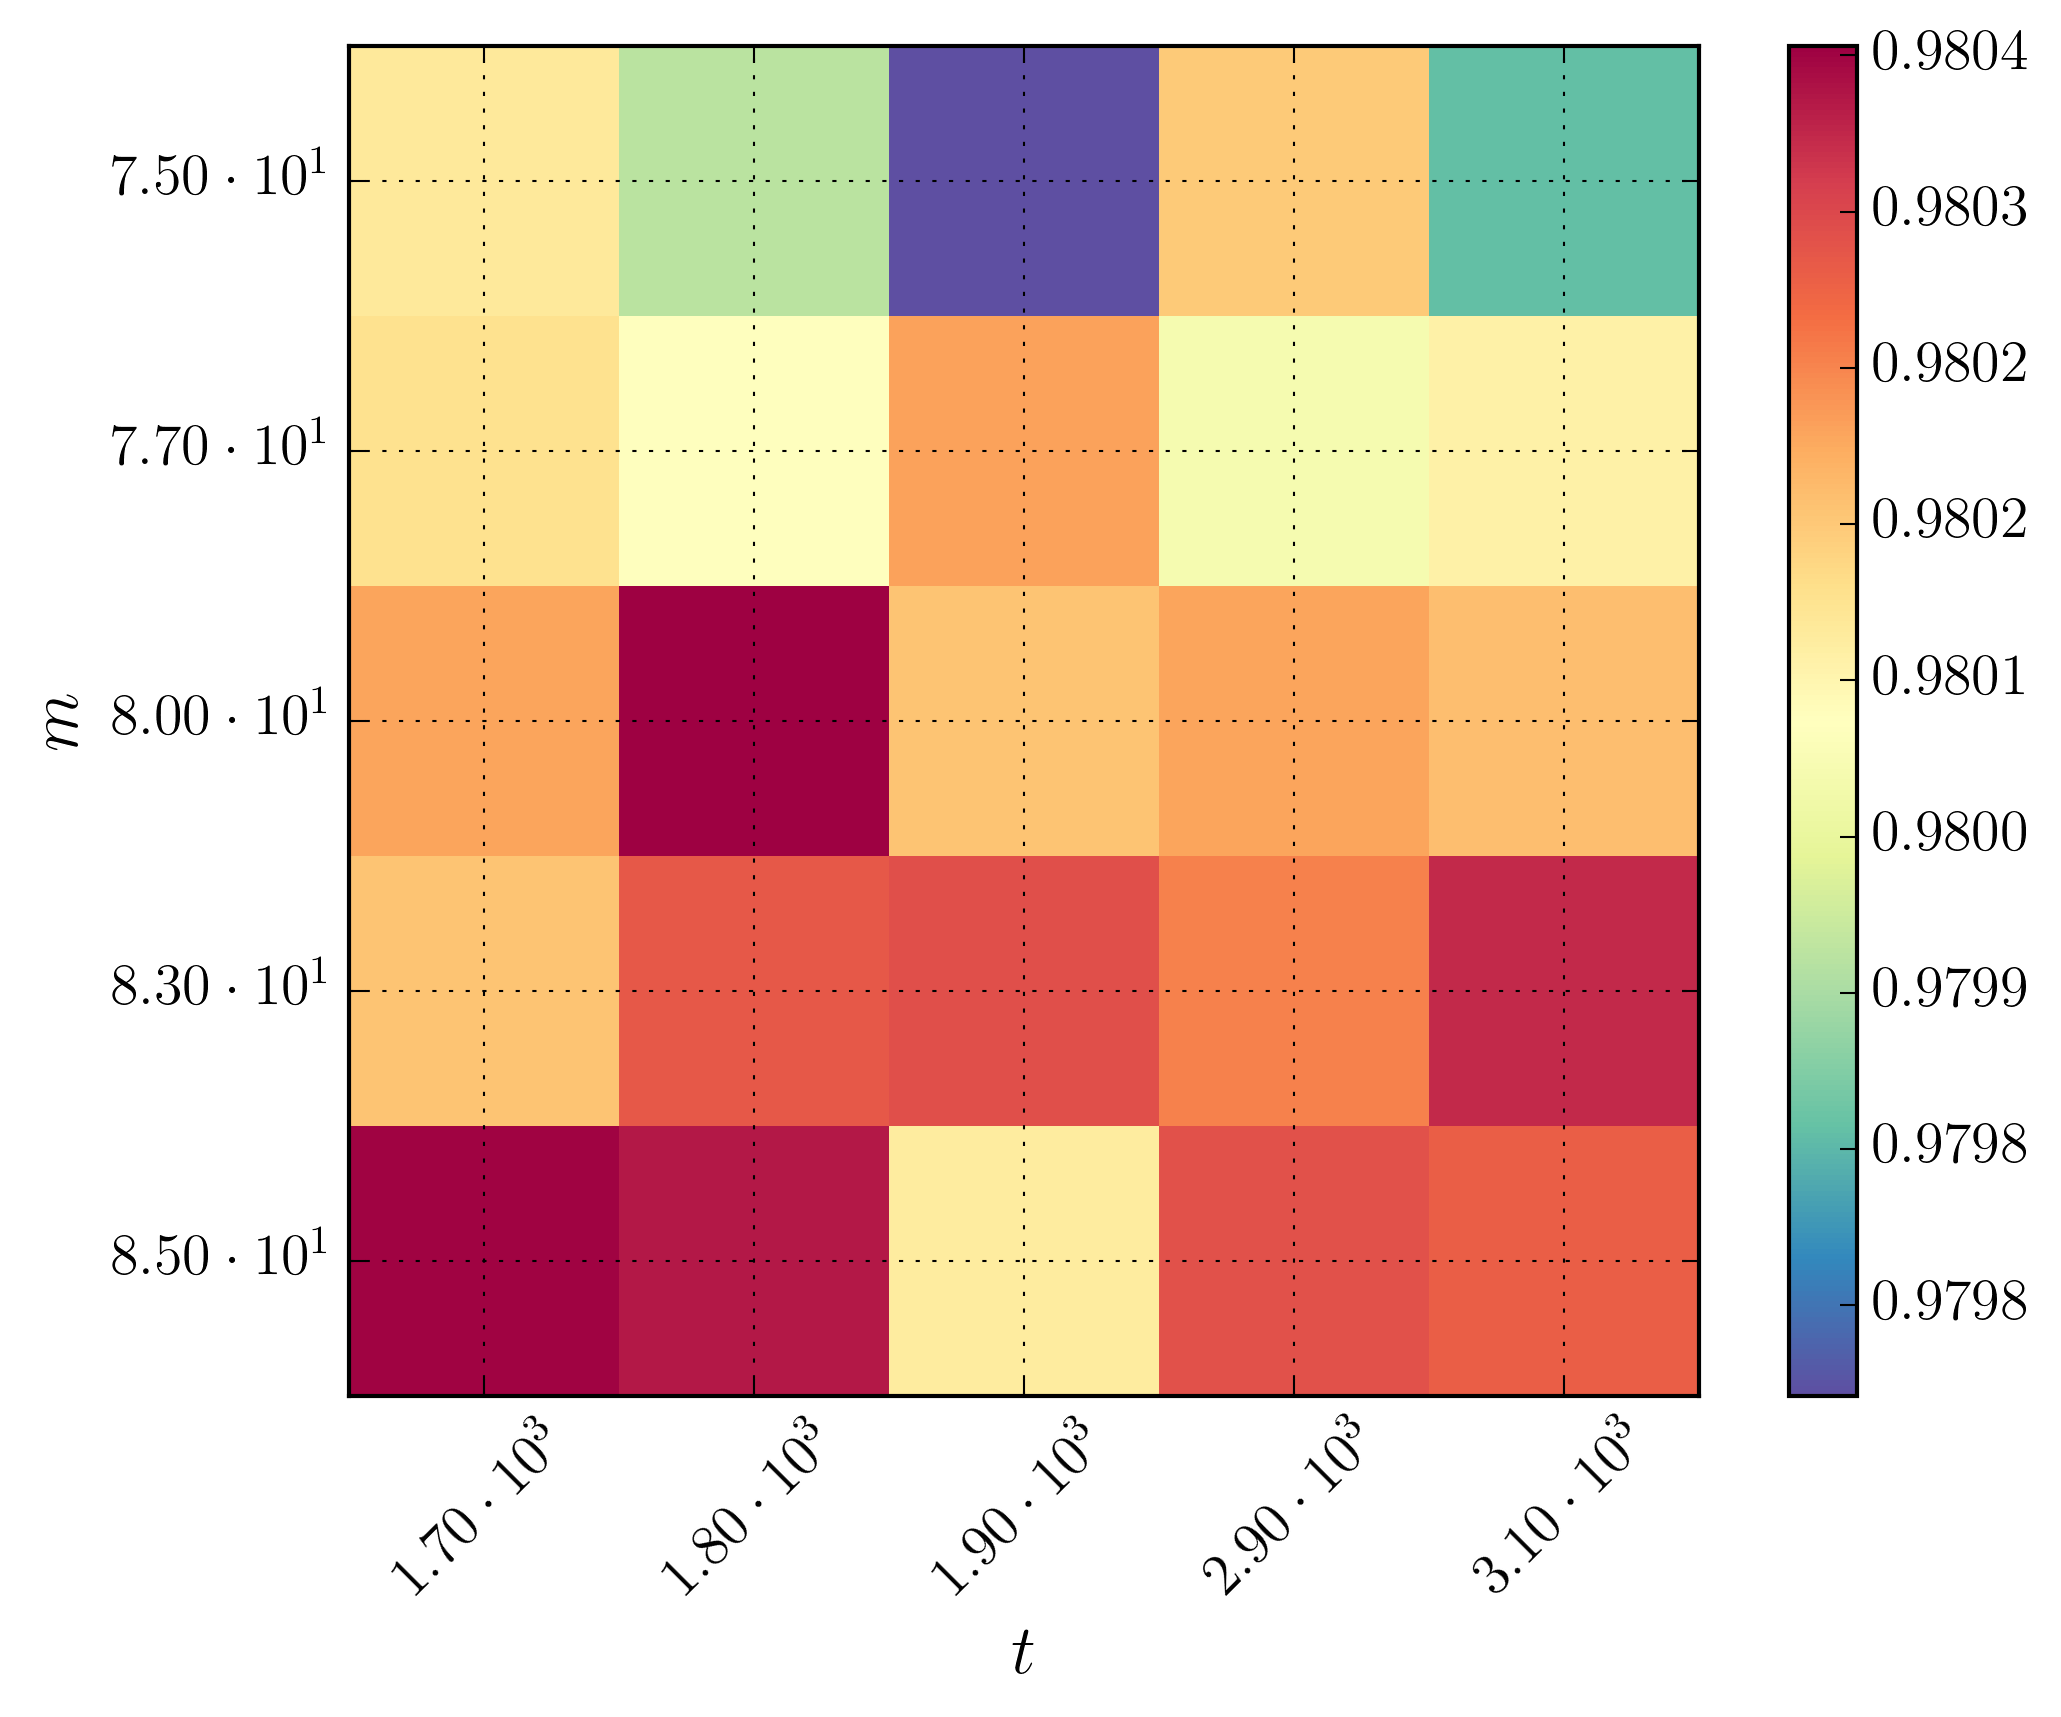
\includegraphics[width=0.51\textwidth,height=0.4\textwidth]{figures/gridsearch/rf/superclasses/rf-superclasses-04.png}}
\caption[Hyperparameter optimization for the Random Forest Classifier]{This figure shows the average, weighted $F_1$ score on the $m$-$t$-plane during the hyperparameter optimization for the Random Forest Classifier, where $t$ is the number of trees in the forest, and $m$ denotes the maximum number of features considered at each split.}
\label{fig:gridsearch-rf-superclasses}
\end{figure}

\renewcommand{\arraystretch}{1.5}
\resizebox{\textwidth}{!}{
\begin{tabular}{c|ccccccccc|c}
\toprule
%& \multicolumn{8 }{c}{Predicted class} & & \\
%\hline
                   & BV        & CEPH       & DSCT      & EB         & LPV         & NoneVar    & QSO       & RRL        & T2CEPH   & $\Sigma $ \\
\hline
BV                 & {\bfseries 773} &            &           &     11     &      3      &      8     &      1    &            &          &     796   \\
CEPH               &     1     & {\bfseries 2226} &           &     18     &      2      &      3     &           &     31     &          &    2281   \\
DSCT               &           &            & {\bfseries 496} &      2     &             &     12     &           &      1     &          &     511   \\
EB                 &     7     &      7     &     2     & {\bfseries 3342} &     52      &     79     &      3    &     43     &     3    &    3538   \\
LPV                &     4     &      2     &           &     10     & {\bfseries 15945} &     32     &      1    &     1      &          &   15995   \\
NoneVar            &    23     &      1     &     4     &     35     &     72      & {\bfseries 4648} &      8    &            &          &    4791   \\
QSO                &           &            &           &      3     &      4      &     25     & {\bfseries 147} &     1      &          &     180   \\
RRL                &           &      9     &     7     &     31     &      2      &     7      &           & {\bfseries 4414} &          &    4470   \\
T2CEPH             &     1     &      15    &           &     19     &      5      &     3      &           &            & {\bf 78} &     121   \\
\bottomrule
Recall ($\%$)      &   97.11   &     97.59  &   97.06   &    94.46   &    99.69    &   97.02    &   81.67   &    98.75   &   64.46  &           \\
\hline
Precision ($\%$)   &   95.55   &     98.50  &   97.45   &    96.28   &    99.13    &   96.49    &   91.87   &    98.29   &   96.93  &           \\
\hline
$F_1$ score ($\%$) &   96.32   &     98.04  &   97.25   &    95.36   &    99.41    &   96.75    &   86.47   &    98.52   &   77.43  & 98.14 $\pm$ 0.07 \\
\bottomrule
\end{tabular}
}

% Hyperparameter optimization
% Add confusion matrix for main classes
% Add confusion matrix for subclasses
% Add feature importance for both

\chapter{Assessing Classification Performance for GAIA}

% Simulating GAIA time series
% Performance of the best classifier on GAIA data